% !TEX program = tectonic
% Slides V2 « La couche données » — NOUVEAU FICHIER, construit d'après PLAN_SLIDES_DONNEES.tex
% (plan validé par Alice 2026-07-16 : une idée par slide, plan annoncé, chronologie,
%  chiffres légendés, zéro mini-détail, choix explicites, public neuf).
% Périmètre : les DONNÉES seulement (Étapes 1-5). Backtest et tables : hors périmètre.
% L'ancien deck SLIDES_DONNEES_S1S2.tex n'est PAS modifié.
% Chiffres : docs/RAPPORT_QUALITE.md (source de vérité) + ANALYSE_FILING_TYPES_HOUSE.md
% + lignée v1-house (01_v1_house/cache/) pour la Cohérence. Figures : docs/{slides,quality,sources}/.
\documentclass[11pt,aspectratio=169]{beamer}
\definecolor{helec}{HTML}{3B6EA5}   % couleur maîtresse (Chambre électronique)
\usetheme{Madrid}
\usecolortheme[named=helec]{structure}
\setbeamertemplate{navigation symbols}{}
\setbeamertemplate{blocks}[rounded][shadow=false]
\setbeamerfont{frametitle}{series=\bfseries}
\usepackage[T1]{fontenc}
\usepackage{lmodern}
\usepackage[utf8]{inputenc}
\usepackage[french]{babel}
\usepackage{booktabs}
\usepackage{xcolor}
\usepackage{graphicx}
\usepackage{amssymb}
\usepackage{amsmath}
\usepackage{array}
\usepackage{newunicodechar}
\usepackage{tikz}
\usetikzlibrary{arrows.meta,positioning,calc}
\hypersetup{colorlinks=true, urlcolor=helec, linkcolor=white}

% Caractères Unicode → commandes (fontes T1)
\newunicodechar{→}{\ensuremath{\rightarrow}}
\newunicodechar{—}{\textemdash}
\newunicodechar{–}{\textendash}
\newunicodechar{…}{\ldots}
\newunicodechar{·}{\textperiodcentered}
\newunicodechar{≈}{\ensuremath{\approx}}
\newunicodechar{×}{\ensuremath{\times}}
\newunicodechar{≤}{\ensuremath{\leq}}
\newunicodechar{≥}{\ensuremath{\geq}}
\newunicodechar{−}{\ensuremath{-}}
\newunicodechar{✓}{\checkmark}
\newunicodechar{↔}{\ensuremath{\leftrightarrow}}
\newunicodechar{œ}{\oe}
\newunicodechar{Œ}{\OE}
\newunicodechar{°}{\textdegree}
\newunicodechar{§}{\S}
\newunicodechar{«}{\og}
\newunicodechar{»}{\fg{}}

% Code couleur des 4 voies
\definecolor{helec}{HTML}{3B6EA5}   % Chambre électronique
\definecolor{hocr}{HTML}{A9C5E2}    % Chambre OCR
\definecolor{selec}{HTML}{8E44AD}   % Sénat électronique
\definecolor{socr}{HTML}{CFAEDE}    % Sénat OCR
\definecolor{okgreen}{HTML}{2E8B57}
\definecolor{alertred}{HTML}{C0392B}
\definecolor{warnorange}{HTML}{E67E22}
\definecolor{dataC}{RGB}{176,110,14}
\definecolor{grisC}{RGB}{90,90,90}

\newcommand{\co}[1]{\texttt{#1}}
\tikzset{
  step/.style={rectangle, rounded corners=2pt, draw=#1, line width=0.8pt, fill=#1!8,
               align=center, font=\scriptsize, minimum height=0.72cm},
  bande/.style={rectangle, rounded corners=2pt, draw=#1, line width=0.8pt, fill=#1!8,
                align=center, font=\scriptsize, minimum height=0.62cm},
  arr/.style={-{Latex[length=2mm]}, line width=0.8pt, draw=gray!65},
}

% Tuile chiffre-clé : \tuile{couleur}{gros chiffre}{légende}
\newcommand{\tuile}[3]{%
  \begin{minipage}[t]{0.23\textwidth}\centering
    \colorbox{#1}{\parbox[c][21mm][c]{\dimexpr\linewidth-8pt}{\centering
      {\color{white}\Large\textbf{#2}}\\[0.6mm]
      {\color{white}\footnotesize #3}}}
  \end{minipage}}

\newcommand{\badge}[2]{\colorbox{#1}{\textcolor{white}{\footnotesize\textbf{#2}}}}
\newcommand{\badgel}[2]{\colorbox{#1}{\textcolor{black!80}{\footnotesize\textbf{#2}}}}

% Carte source : \carte{couleur}{titre}{contenu}
\newcommand{\carte}[3]{%
  \colorbox{#1!10}{\parbox[t][23mm][t]{\dimexpr\linewidth-8pt}{\vspace{1mm}
    {\color{#1}\footnotesize\textbf{#2}}\\[0.8mm]{\scriptsize #3}}}}

% Encadré CHOIX (un choix méthodologique, énoncé en une phrase)
\newcommand{\choixbox}[1]{%
  \colorbox{alertred!8}{\parbox{\dimexpr\linewidth-8pt}{\scriptsize
    \textbf{\textcolor{alertred}{CHOIX}}\; --- #1}}}

% Bandeau RÉPONSE (dernière slide de chaque étape)
\newcommand{\repband}[1]{%
  \colorbox{okgreen!12}{\parbox{\dimexpr\textwidth-10pt}{\scriptsize
    \textbf{\textcolor{okgreen}{Réponse}}\; --- #1}}}

\title[La couche données]{La couche données --- collecte \& validation}
\subtitle{Transactions boursières du Congrès américain · Chambre \& Sénat · 2014--2026}
\author[A.~Lemaire]{Alice Lemaire}
\institute[Ramify]{Document de recherche --- livrable Ramify}
\date{Juillet 2026}

\begin{document}

% ── Titre ──
\begin{frame}[plain]
  \titlepage
\end{frame}

% ══════════════════ OUVERTURE ══════════════════

% ── O1 · Le pourquoi (NEUVE) ──
\begin{frame}{Depuis 2012, chaque élu du Congrès doit déclarer ses transactions en bourse}
  \centering
  {\normalsize le \textbf{STOCK Act} (2012) : toute transaction boursière de plus de
   1\,000~\$ d'un élu doit être déclarée dans un\\
   \emph{Periodic Transaction Report} (« \textbf{PTR} ») --- public, daté, sous
   \textbf{45 jours}}\\[5mm]
  \tuile{helec}{45 j}{le délai légal pour\\déclarer un trade}\hfill
  \tuile{grisC}{2014--2026}{la fenêtre étudiée\\(la loi date de 2012)}\hfill
  \tuile{dataC}{2 chambres}{435 représentants\\+ 100 sénateurs}\\[5mm]
  \colorbox{helec!10}{\parbox{0.86\textwidth}{\centering\footnotesize\vspace{0.8mm}
    \textbf{la question de recherche} : ces déclarations publiques peuvent-elles nourrir
    une stratégie d'investissement ?\\
    avant d'y répondre, il faut une donnée \textbf{complète, propre et prouvée} ---
    c'est l'objet de cette présentation\vspace{0.8mm}}}
\end{frame}

% ── O2 · Les 4 résultats d'abord (NEUVE) ──
\begin{frame}{La couche données, en quatre résultats}
  \centering
  \vspace{4mm}
  \tuile{grisC}{169\,000}{transactions uniques,\\identité rattachée à 100\,\%}\hfill
  \tuile{helec}{100\,\%}{des 8\,252 déclarations\\officielles (PTR) traitées}\hfill
  \tuile{alertred}{$>$\,92\,\%}{base du tiers retrouvée · 87,8\,\%\\des positions expliquées}\hfill
  \tuile{okgreen}{134\,464 $\times$ 36}{la table de recherche\\livrée, limites écrites}\\[8mm]
  {\footnotesize\color{black!70} comment peut-on affirmer tout ça ?
   --- c'est l'objet de la présentation : chaque étape prouve son chiffre}
\end{frame}

% ── O3 · Le plan : cinq étapes (refonte S1) ──
\begin{frame}{Le plan --- cinq étapes, une promesse}
  \centering
  \vspace{3mm}
  \begin{tikzpicture}[scale=1.0, every node/.style={transform shape}]
\node[rectangle, rounded corners=2.5pt, draw=helec, fill=helec!10, line width=0.8pt, text width=2.35cm, minimum height=1.05cm, align=center, font=\scriptsize] (b1) at (1.325,0) {\color{helec}\textbf{1 · \mbox{Donnée brute}}};
\node[below=1.2mm of b1, align=center, font=\tiny, text=black!60] {Chambre \& Sénat :\\à quoi ça ressemble};
\draw[arr] (2.65,0) -- (3.07,0);
\node[rectangle, rounded corners=2.5pt, draw=grisC, fill=grisC!10, line width=0.8pt, text width=2.35cm, minimum height=1.05cm, align=center, font=\scriptsize] (b2) at (4.395,0) {\color{grisC}\textbf{2 · Pipeline}};
\node[below=1.2mm of b2, align=center, font=\tiny, text=black!60] {4 voies\\d'extraction};
\draw[arr] (5.72,0) -- (6.14,0);
\node[rectangle, rounded corners=2.5pt, draw=dataC, fill=dataC!10, line width=0.8pt, text width=2.35cm, minimum height=1.05cm, align=center, font=\scriptsize] (b3) at (7.465,0) {\color{dataC}\textbf{3 · Enrichir}};
\node[below=1.2mm of b3, align=center, font=\tiny, text=black!60] {tickers · secteurs\\· dédoublonnage};
\draw[arr] (8.79,0) -- (9.209999999999999,0);
\node[rectangle, rounded corners=2.5pt, draw=alertred, fill=alertred!10, line width=1.3pt, text width=2.75cm, minimum height=1.05cm, align=center, font=\scriptsize] (b4) at (10.735,0) {\color{alertred}\textbf{4 · \mbox{VÉRIFICATION}}};
\node[below=1.2mm of b4, align=center, font=\tiny, text=black!60] {complétude · cohérence\\· corroboration};
\draw[arr] (12.259999999999998,0) -- (12.679999999999998,0);
\node[rectangle, rounded corners=2.5pt, draw=okgreen, fill=okgreen!10, line width=0.8pt, text width=2.35cm, minimum height=1.05cm, align=center, font=\scriptsize] (b5) at (14.004999999999999,0) {\color{okgreen}\textbf{5 · Livrable}};
\node[below=1.2mm of b5, align=center, font=\tiny, text=black!60] {la table livrée\\+ limites écrites};
\end{tikzpicture}\\[12mm]
  {\footnotesize\color{black!55} chaque étape s'ouvre sur une \textbf{question} et se ferme
   sur une \textbf{réponse chiffrée} --- les choix faits sont encadrés
   \badge{alertred}{CHOIX} au fil des slides}
\end{frame}

\section{Étape 1 · La donnée brute}
% ── intercalaire Étape 1 ──
\begin{frame}[plain]
  \centering
  \vspace{14mm}
  {\Large\bfseries\color{black!80} Étape 1 --- La donnée brute}\\[8mm]
  \begin{tikzpicture}[scale=1.0, every node/.style={transform shape}]
\node[rectangle, rounded corners=2.5pt, draw=helec, fill=helec, line width=0.8pt, text width=2.35cm, minimum height=1.05cm, align=center, font=\scriptsize] (b1) at (1.325,0) {\color{white}\textbf{1 · \mbox{Donnée brute}}};
\draw[arr] (2.65,0) -- (3.07,0);
\node[rectangle, rounded corners=2.5pt, draw=grisC, fill=grisC!10, line width=0.8pt, text width=2.35cm, minimum height=1.05cm, align=center, font=\scriptsize] (b2) at (4.395,0) {\color{grisC}\textbf{2 · Pipeline}};
\draw[arr] (5.72,0) -- (6.14,0);
\node[rectangle, rounded corners=2.5pt, draw=dataC, fill=dataC!10, line width=0.8pt, text width=2.35cm, minimum height=1.05cm, align=center, font=\scriptsize] (b3) at (7.465,0) {\color{dataC}\textbf{3 · Enrichir}};
\draw[arr] (8.79,0) -- (9.209999999999999,0);
\node[rectangle, rounded corners=2.5pt, draw=alertred, fill=alertred!10, line width=1.3pt, text width=2.75cm, minimum height=1.05cm, align=center, font=\scriptsize] (b4) at (10.735,0) {\color{alertred}\textbf{4 · \mbox{VÉRIFICATION}}};
\draw[arr] (12.259999999999998,0) -- (12.679999999999998,0);
\node[rectangle, rounded corners=2.5pt, draw=okgreen, fill=okgreen!10, line width=0.8pt, text width=2.35cm, minimum height=1.05cm, align=center, font=\scriptsize] (b5) at (14.004999999999999,0) {\color{okgreen}\textbf{5 · Livrable}};
\end{tikzpicture}\\[9mm]
  {\normalsize\itshape\color{black!55} À quoi ressemble la matière première ---
   et pourquoi ce n'est pas juste télécharger un CSV ?}
\end{frame}

% ── 1.1 · Deux guichets (fusion S2a+S2b+S7a+S7b) ──
\begin{frame}{Tout est public : deux guichets, treize années}
  \begin{columns}[T]
    \begin{column}{0.48\textwidth}\centering
      \fcolorbox{black!25}{white}{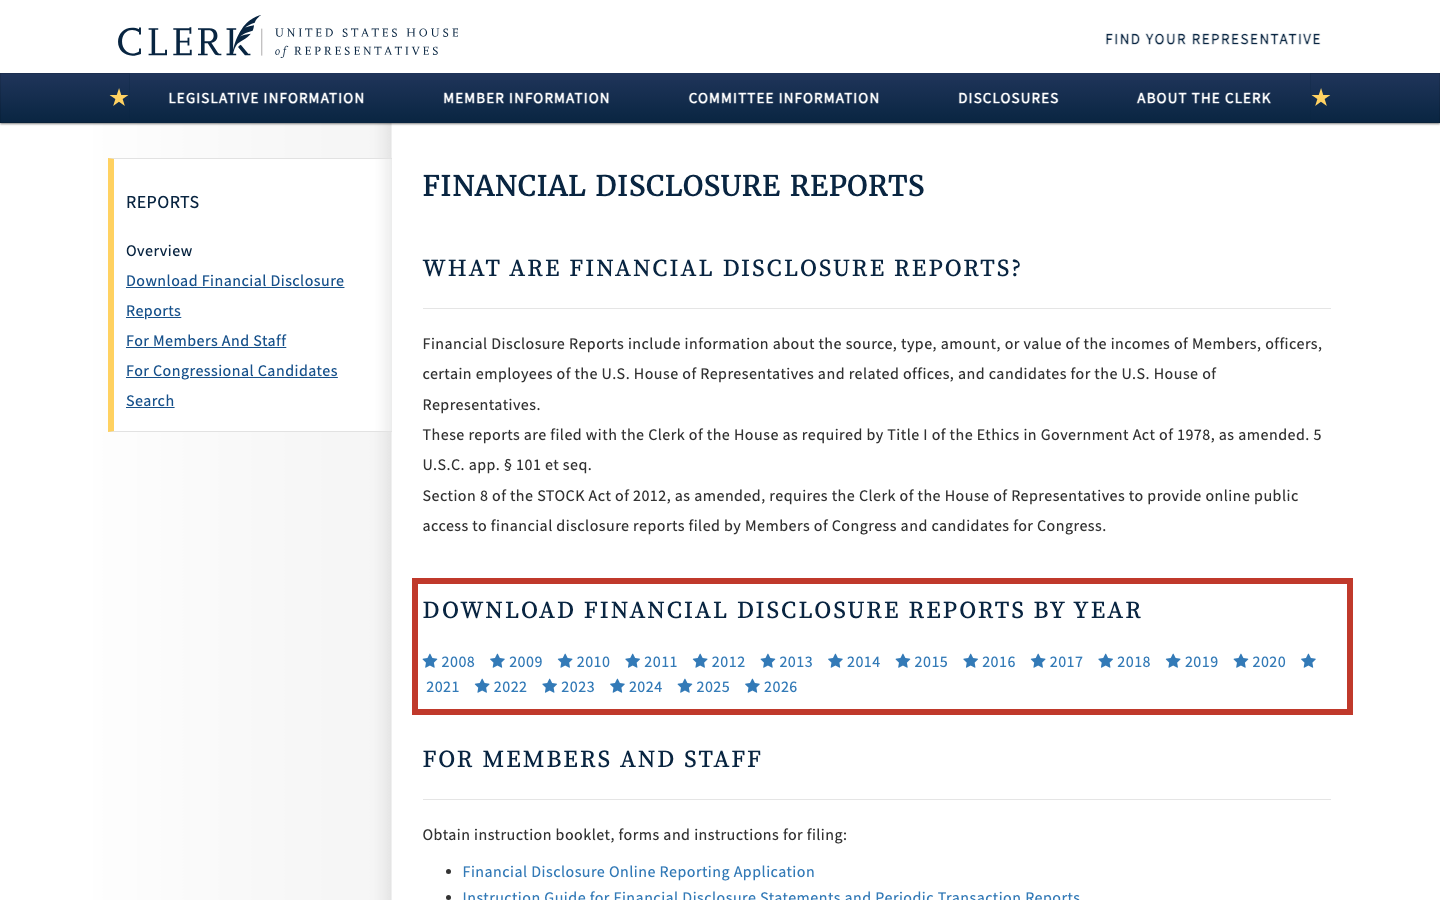
\includegraphics[width=0.93\linewidth,height=36mm,keepaspectratio]{slides/site_house_clerk.png}}\\[0.8mm]
      {\footnotesize\textbf{La Chambre} --- \href{https://disclosures-clerk.house.gov/FinancialDisclosure}{\texttt{disclosures-clerk.house.gov}}}\\[0.3mm]
      {\scriptsize une \textbf{archive par année}, avec l'\textbf{index} de tous les dépôts}
    \end{column}
    \begin{column}{0.48\textwidth}\centering
      \fcolorbox{black!25}{white}{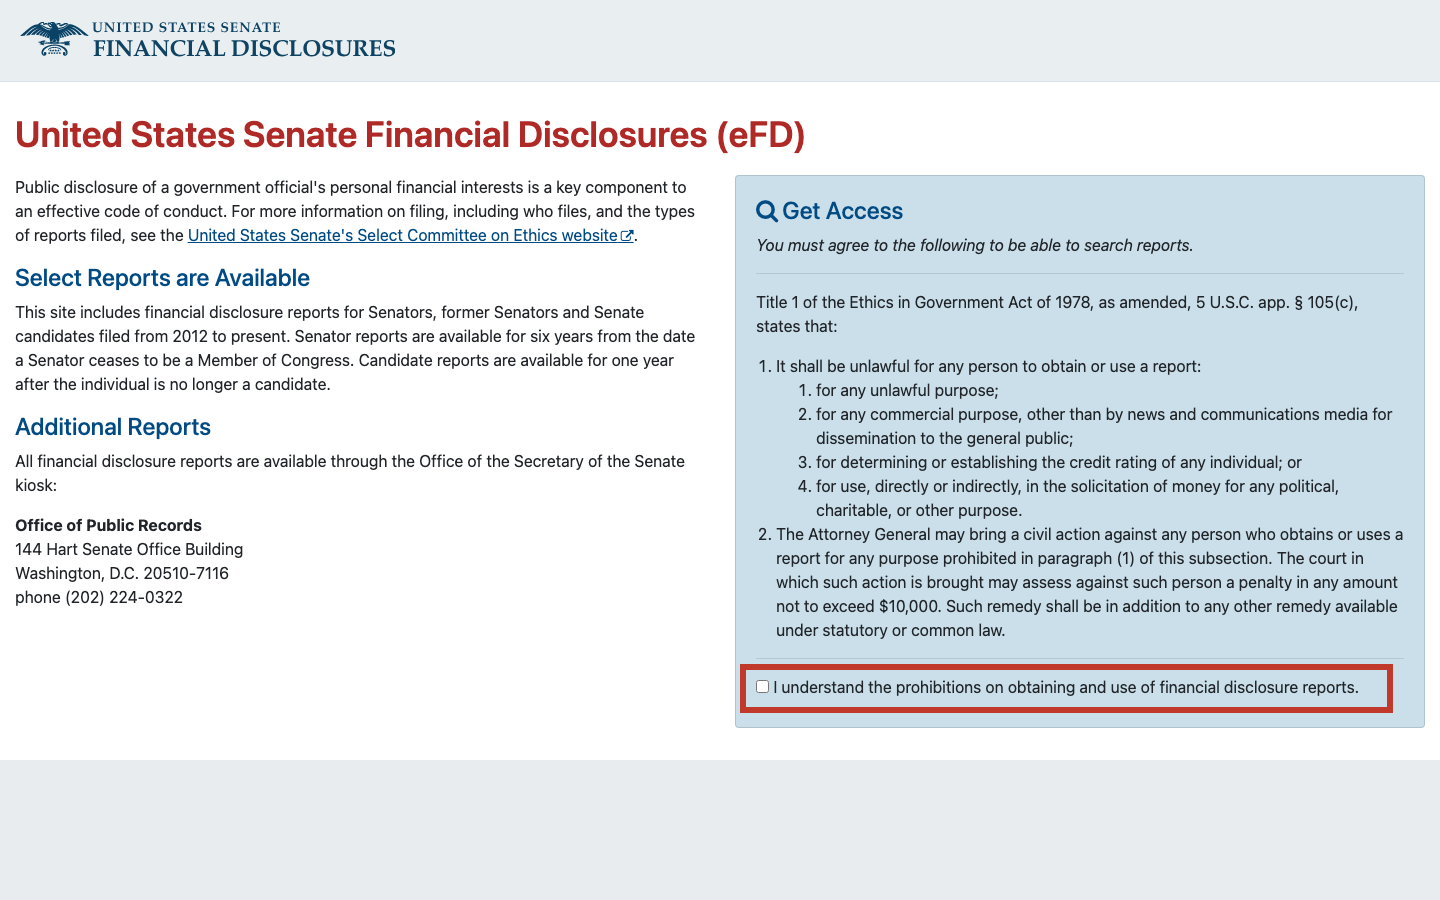
\includegraphics[width=0.93\linewidth,height=36mm,keepaspectratio]{slides/site_senate_efd.png}}\\[0.8mm]
      {\footnotesize\textbf{Le Sénat} --- \emph{efdsearch.senate.gov} (portail eFD)}\\[0.3mm]
      {\scriptsize un \textbf{accord obligatoire}, puis une recherche : la liste des
       dépôts, un lien chacun}
    \end{column}
  \end{columns}
  \vspace{1.5mm}
  \centering
  {\footnotesize \textbf{35\,315} dépôts de tous types dans l'index Chambre ·
   \textbf{13 années} couvertes (2014--2026) · collecte \textbf{automatisée} des deux côtés}\\[1mm]
  \choixbox{l'\textbf{index annuel officiel est notre autorité} : c'est lui qui définit
   l'univers des documents à traiter --- pas ce qu'on a réussi à lire.}
\end{frame}

% ── 1.2 · Le filtre P (S3 conservée) ──
\begin{frame}{Sur douze types de dépôts, un seul porte le signal : le \texttt{P}}
  \centering
  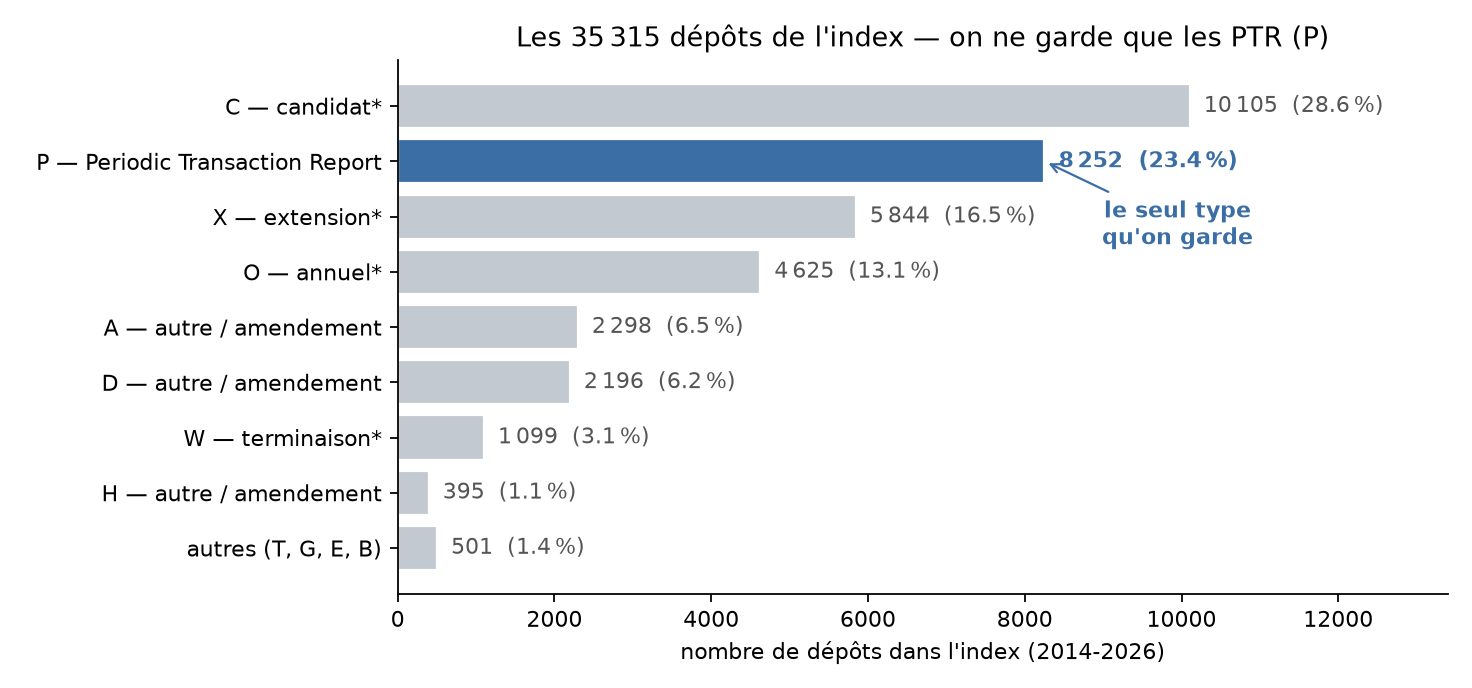
\includegraphics[width=0.70\textwidth]{slides/fig_filingtypes.png}\\[1mm]
  {\footnotesize \textbf{P} = \emph{Periodic Transaction Report} (les « PTR ») --- les
   seules \textbf{déclarations de transactions datées}, sous 45 jours ·
   \textbf{8\,252} PTR parmi les 35\,315 dépôts}\\[1.2mm]
  \choixbox{on ne construit le signal qu'avec les dépôts de type \textbf{P}, parce
   qu'eux seuls déclarent des transactions datées sous 45 jours --- les \textbf{11
   autres types seront tous ouverts} à l'Étape 4 (Vérification).}
\end{frame}

% ── 1.3 · Quatre sous-corpus (fusion S4+S7c+S8) ──
\begin{frame}{Chaque dépôt s'ouvre dans un des deux mondes --- texte ou image : quatre sous-corpus}
  \centering
  {\footnotesize chaque dépôt pointe vers son document (son numéro donne l'URL) ---
   la même donnée réglementaire existe sous \textbf{4 formats} :}\\[1.2mm]
  \begin{columns}[T]
    \begin{column}{0.24\textwidth}\centering
      \fcolorbox{helec}{white}{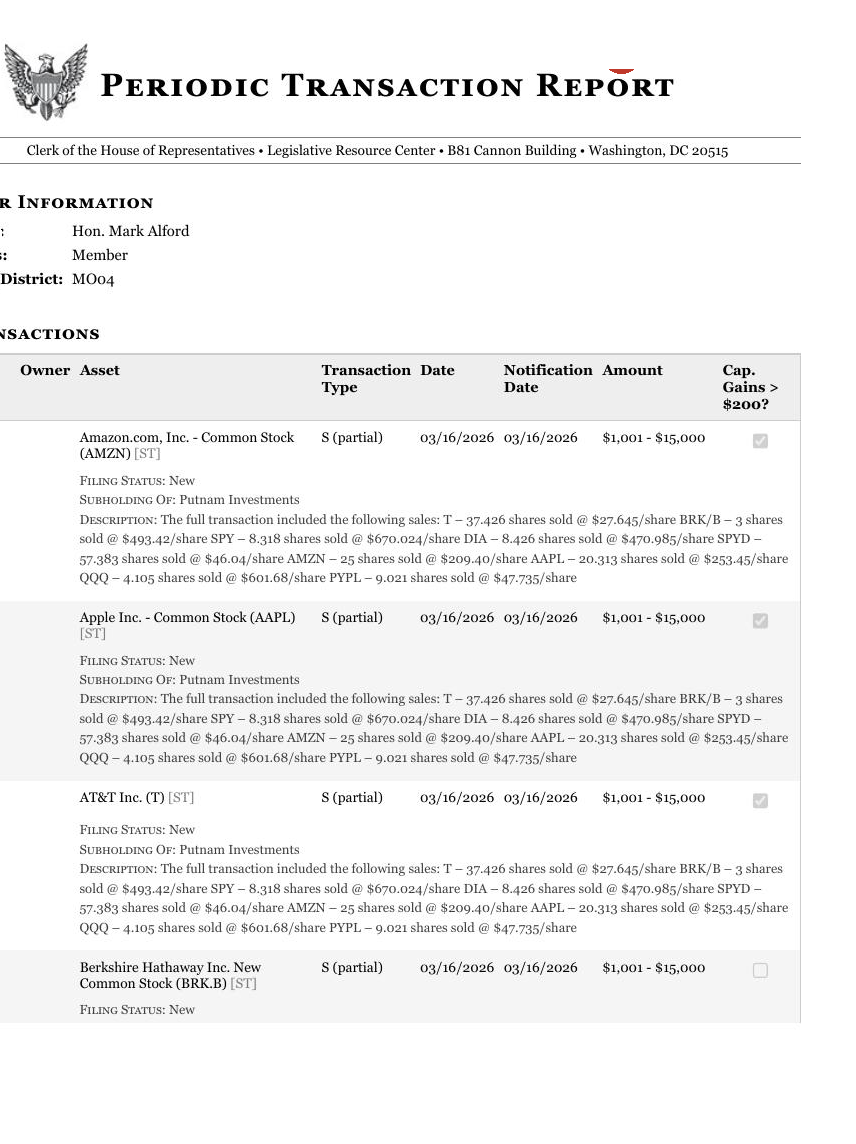
\includegraphics[width=0.88\linewidth,height=27mm,keepaspectratio]{sources/house_digital.png}}\\[0.8mm]
      \badge{helec}{Chambre · PDF lisible}\\[0.4mm]
      {\scriptsize couche texte --- \textbf{71\,\%} des dépôts}
    \end{column}
    \begin{column}{0.24\textwidth}\centering
      \fcolorbox{hocr}{white}{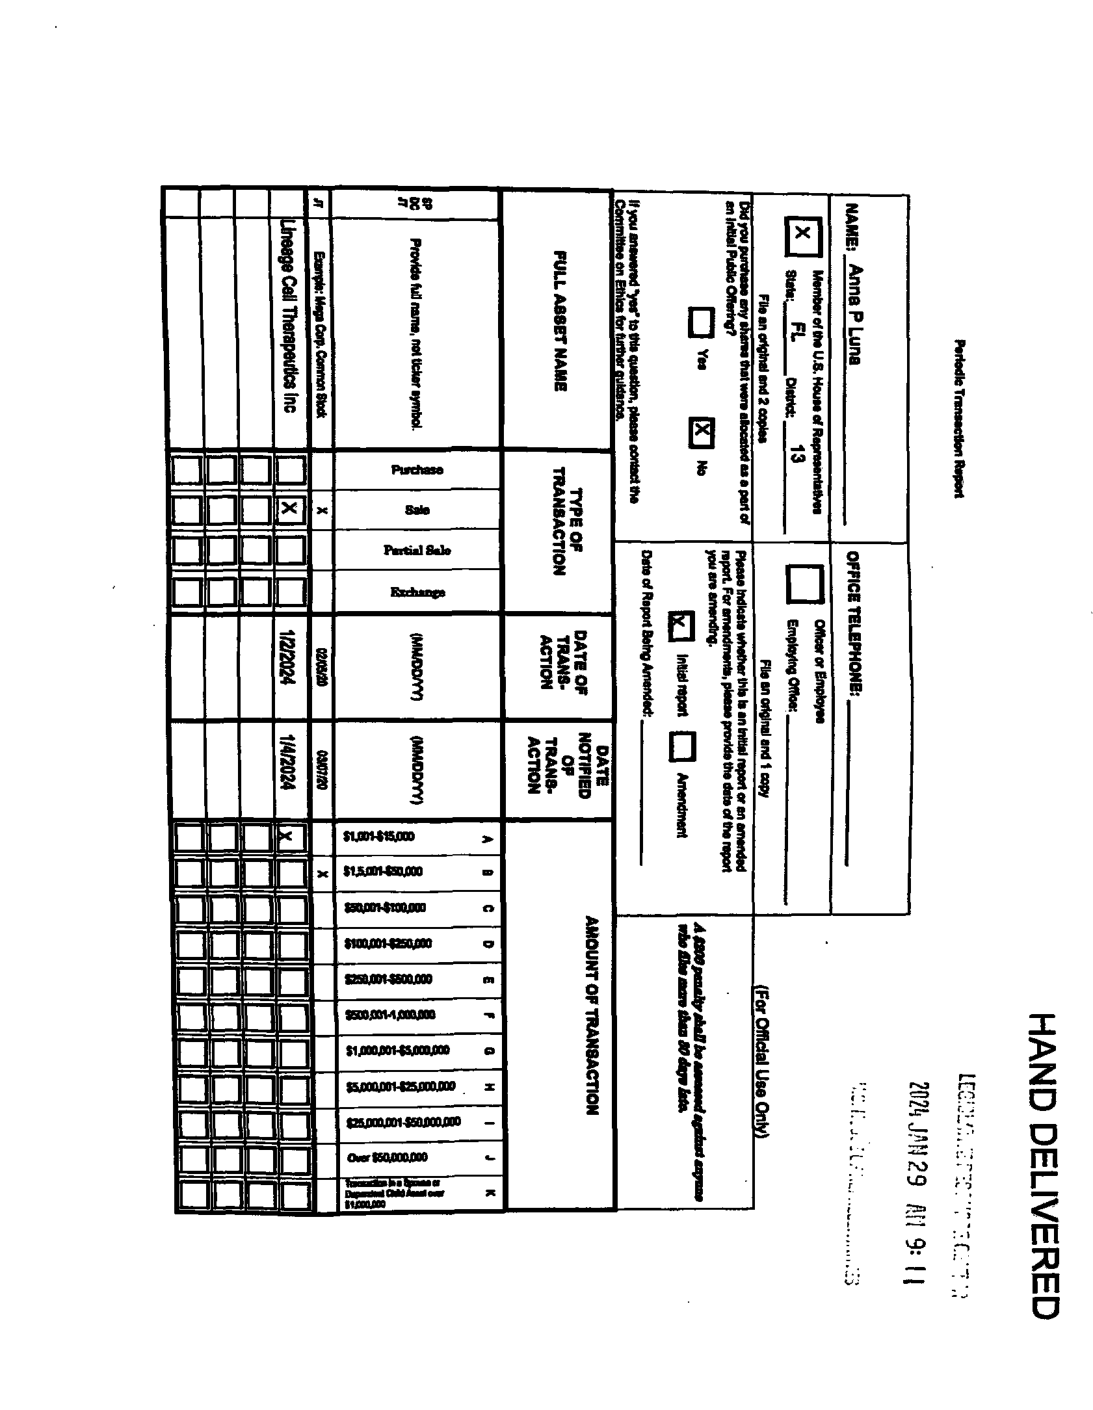
\includegraphics[width=0.88\linewidth,height=27mm,keepaspectratio]{sources/house_ocr.png}}\\[0.8mm]
      \badgel{hocr}{Chambre · PDF scanné}\\[0.4mm]
      {\scriptsize image --- \textbf{29\,\%} des dépôts}
    \end{column}
    \begin{column}{0.24\textwidth}\centering
      \fcolorbox{selec}{white}{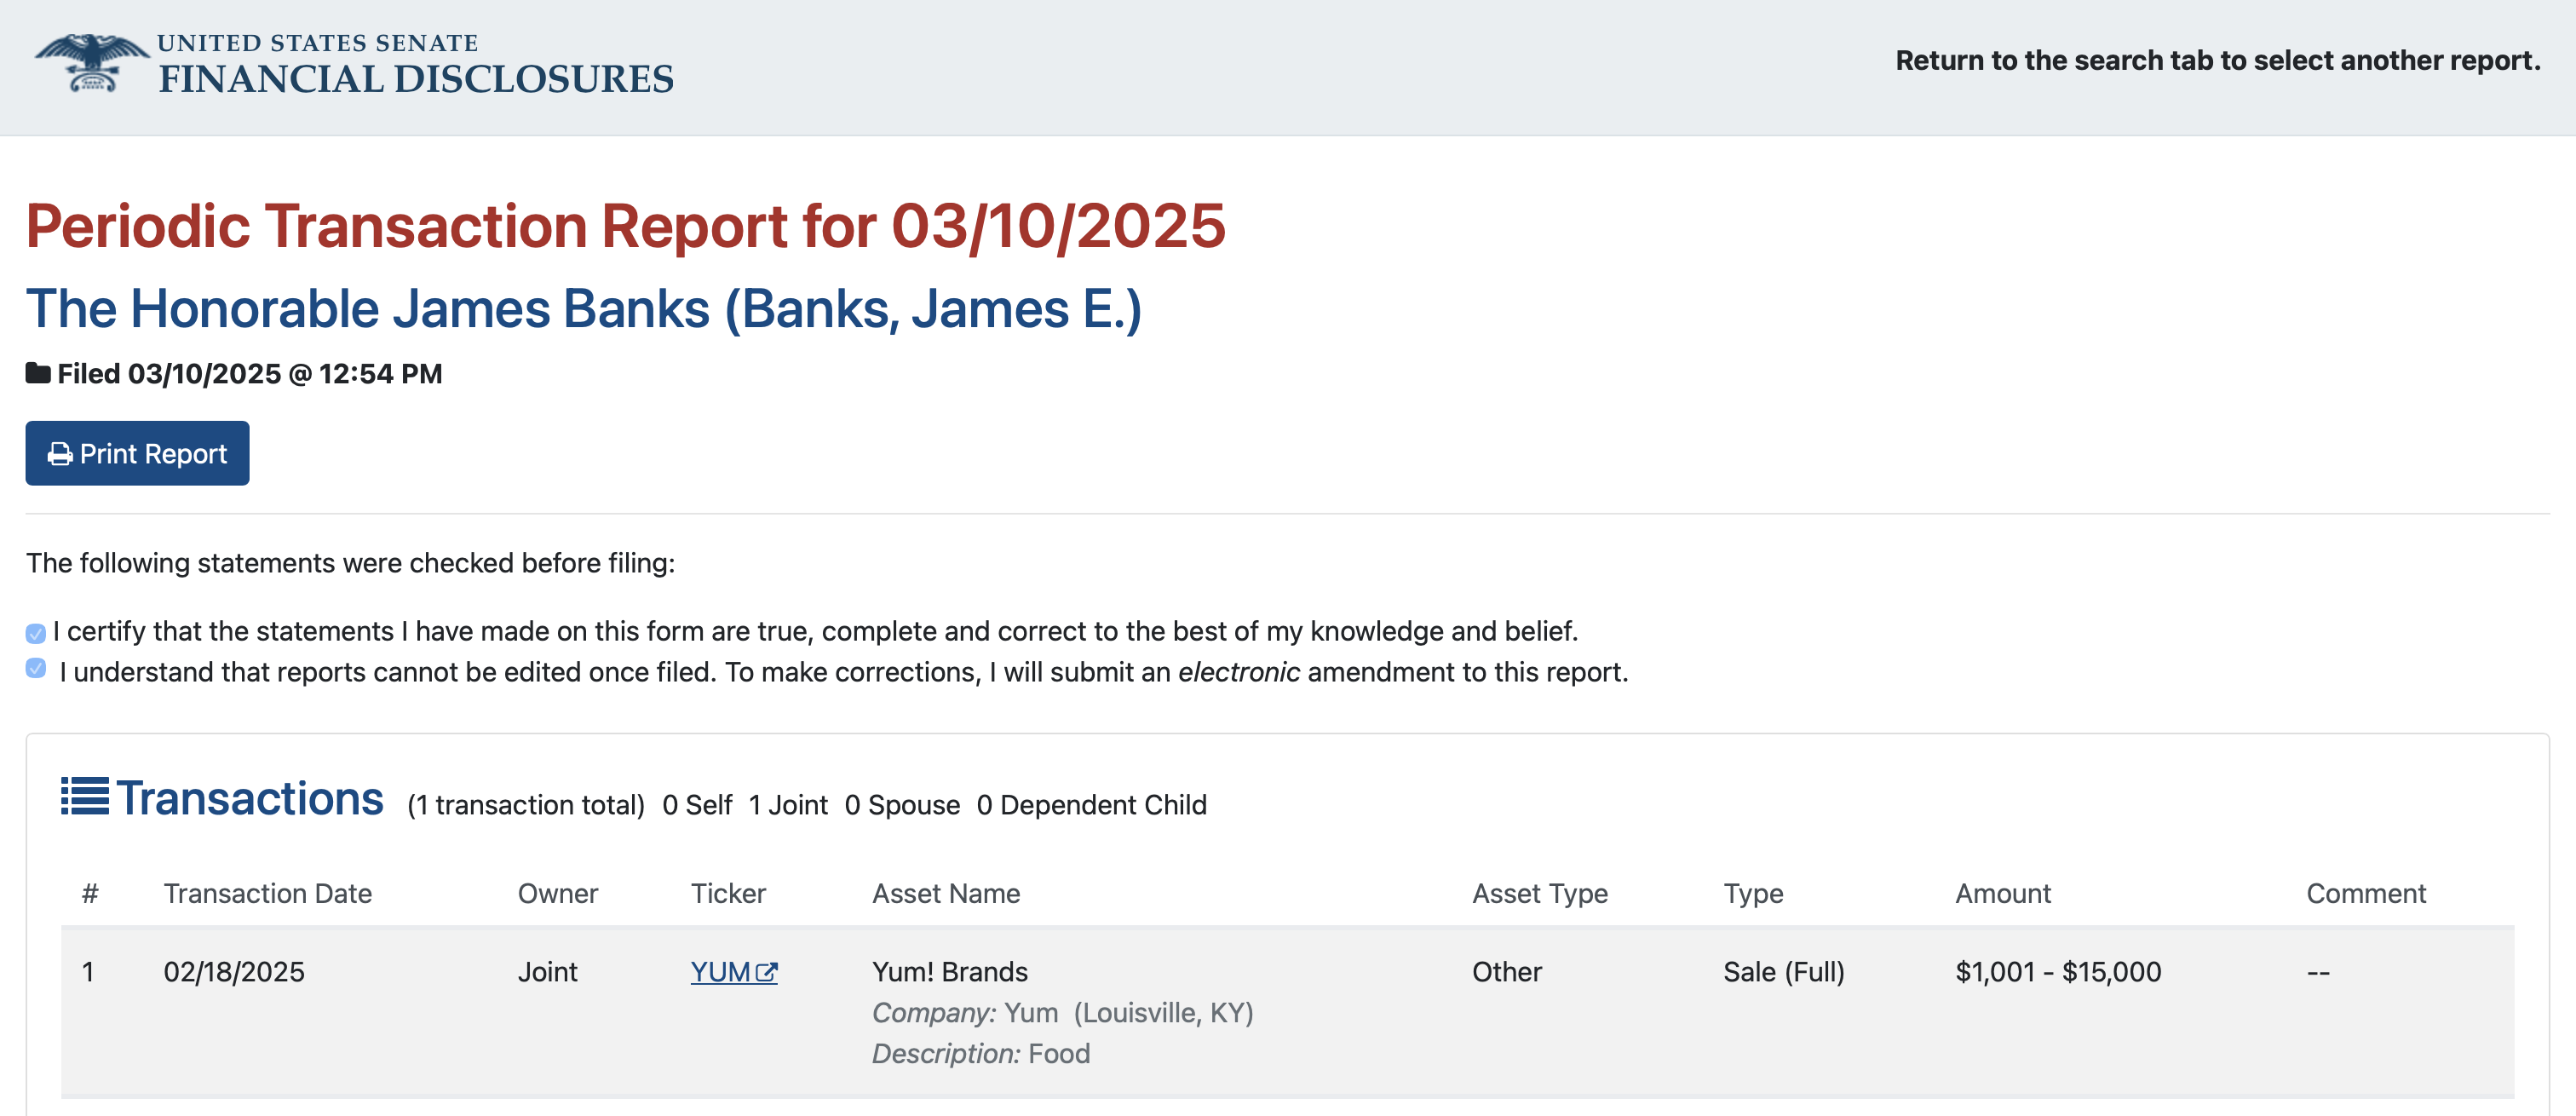
\includegraphics[width=0.88\linewidth,height=27mm,keepaspectratio]{sources/senate_digital.png}}\\[0.8mm]
      \badge{selec}{Sénat · page HTML}\\[0.4mm]
      {\scriptsize table propre, en ligne}
    \end{column}
    \begin{column}{0.24\textwidth}\centering
      \fcolorbox{socr}{white}{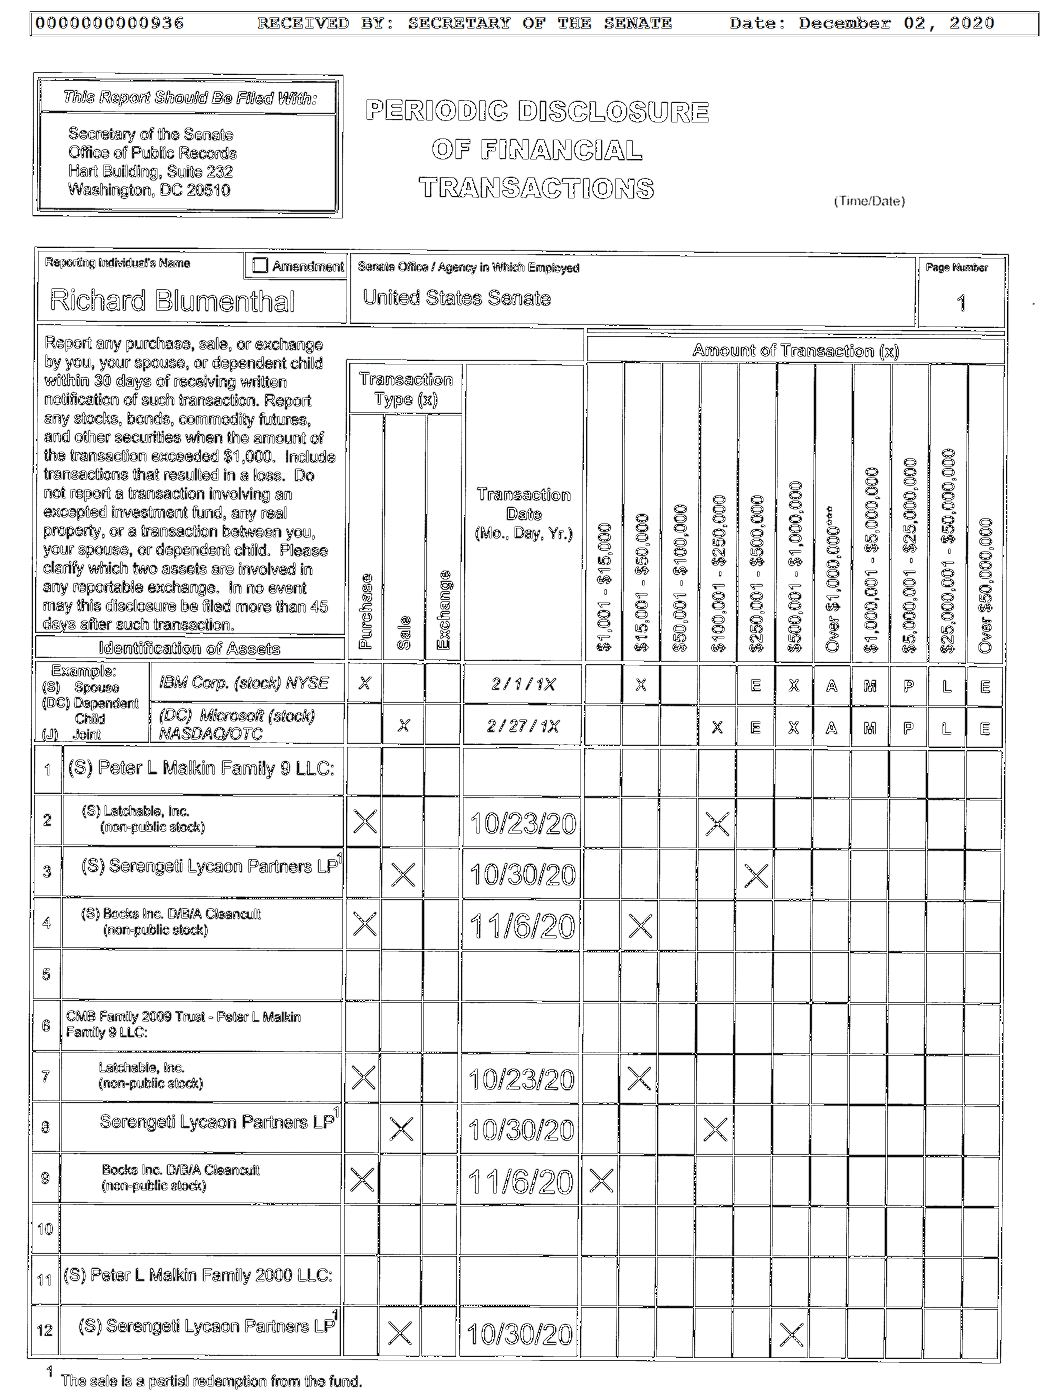
\includegraphics[width=0.88\linewidth,height=27mm,keepaspectratio]{slides/senat_papier_droit.png}}\\[0.8mm]
      \badgel{socr}{Sénat · papier scanné}\\[0.4mm]
      {\scriptsize formulaire, image}
    \end{column}
  \end{columns}
  \vspace{2.5mm}
  \choixbox{on découpe le corpus en \textbf{4 sous-corpus} (chambre × format) et chaque
   voie reçoit son \textbf{extracteur dédié} --- un traitement uniforme raterait la
   moitié · au final, \textbf{57,6\,\%} du corpus viendra d'images.}
\end{frame}

% ── 1.4 · Le manuscrit, point dur (S6 conservée) ──
\begin{frame}{Le vrai point dur n'est pas le scan : c'est le manuscrit}
  \centering
  {\footnotesize un scan n'est pas du texte, c'est une \textbf{image} (à lire par
   \textbf{OCR} : lecture automatique) --- ce qui compte n'est pas l'orientation mais
   \textbf{tapé vs manuscrit} :}\\[2.5mm]
  \begin{columns}[T]
    \begin{column}{0.37\textwidth}\centering
      \fcolorbox{black!30}{white}{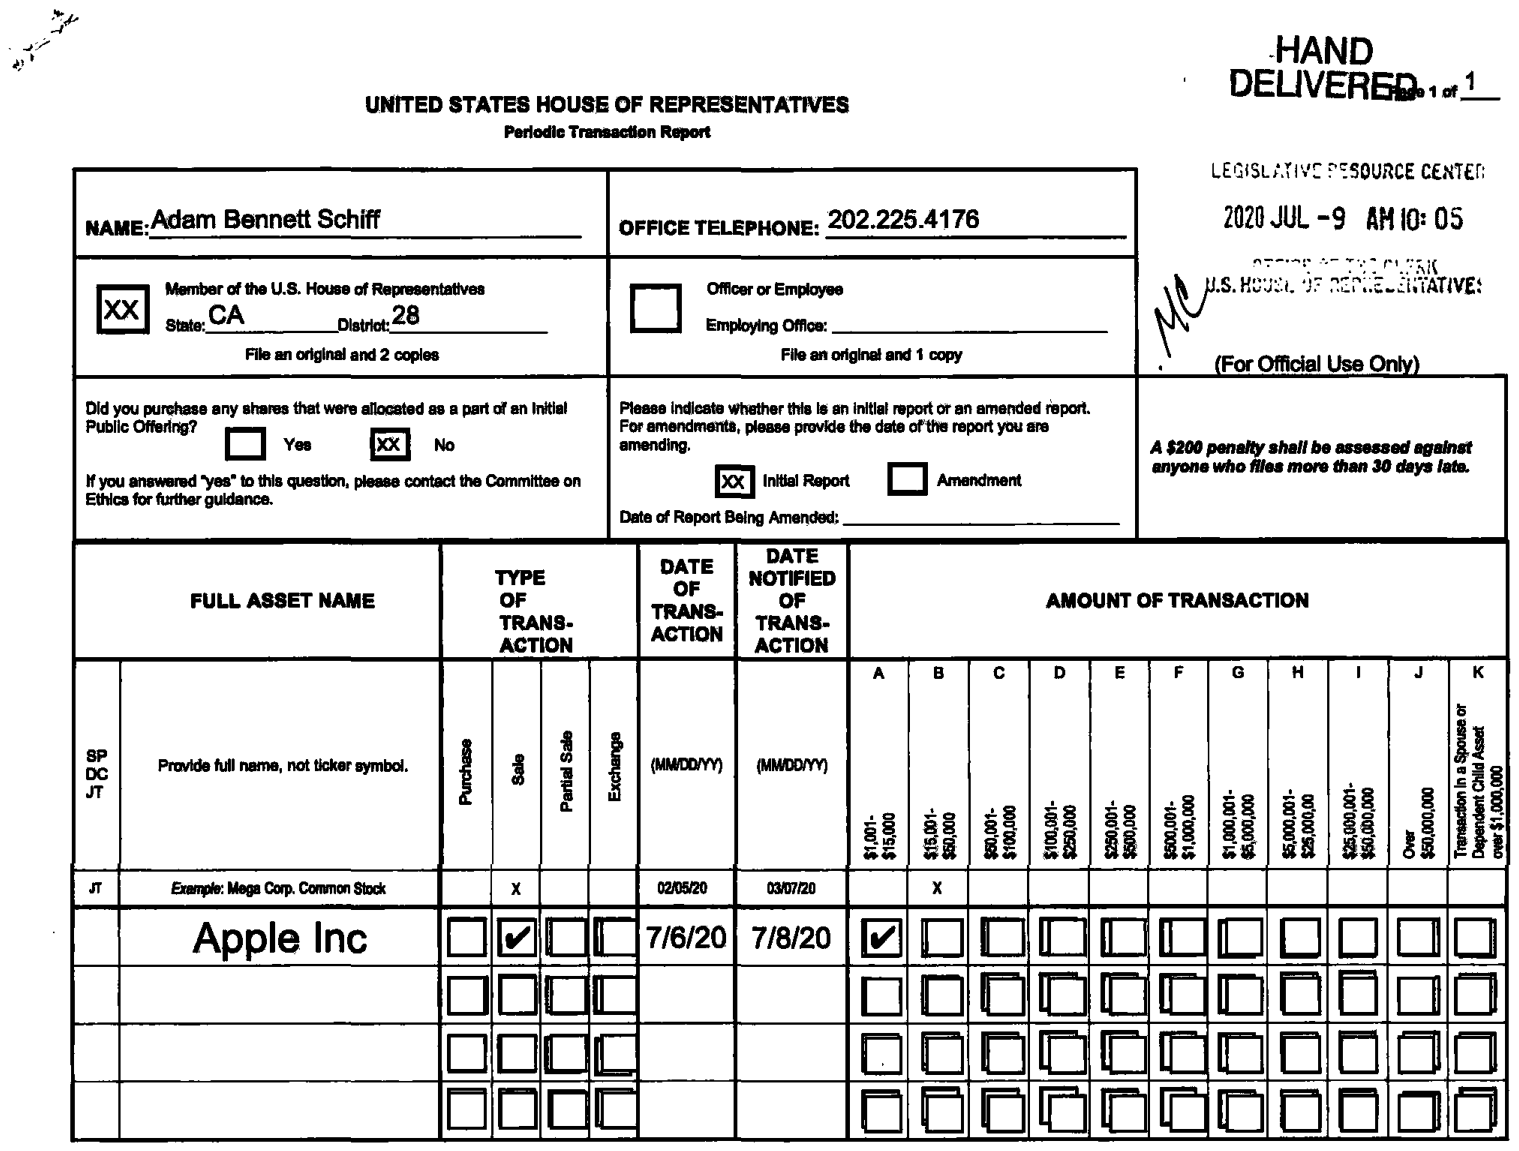
\includegraphics[height=31mm]{slides/scan_full_droit.png}}\\[1mm]
      {\footnotesize\textbf{Tapé, droit}}\\[0.3mm]
      {\scriptsize dactylographié, lisible tel quel}
    \end{column}
    \begin{column}{0.21\textwidth}\centering
      \fcolorbox{black!30}{white}{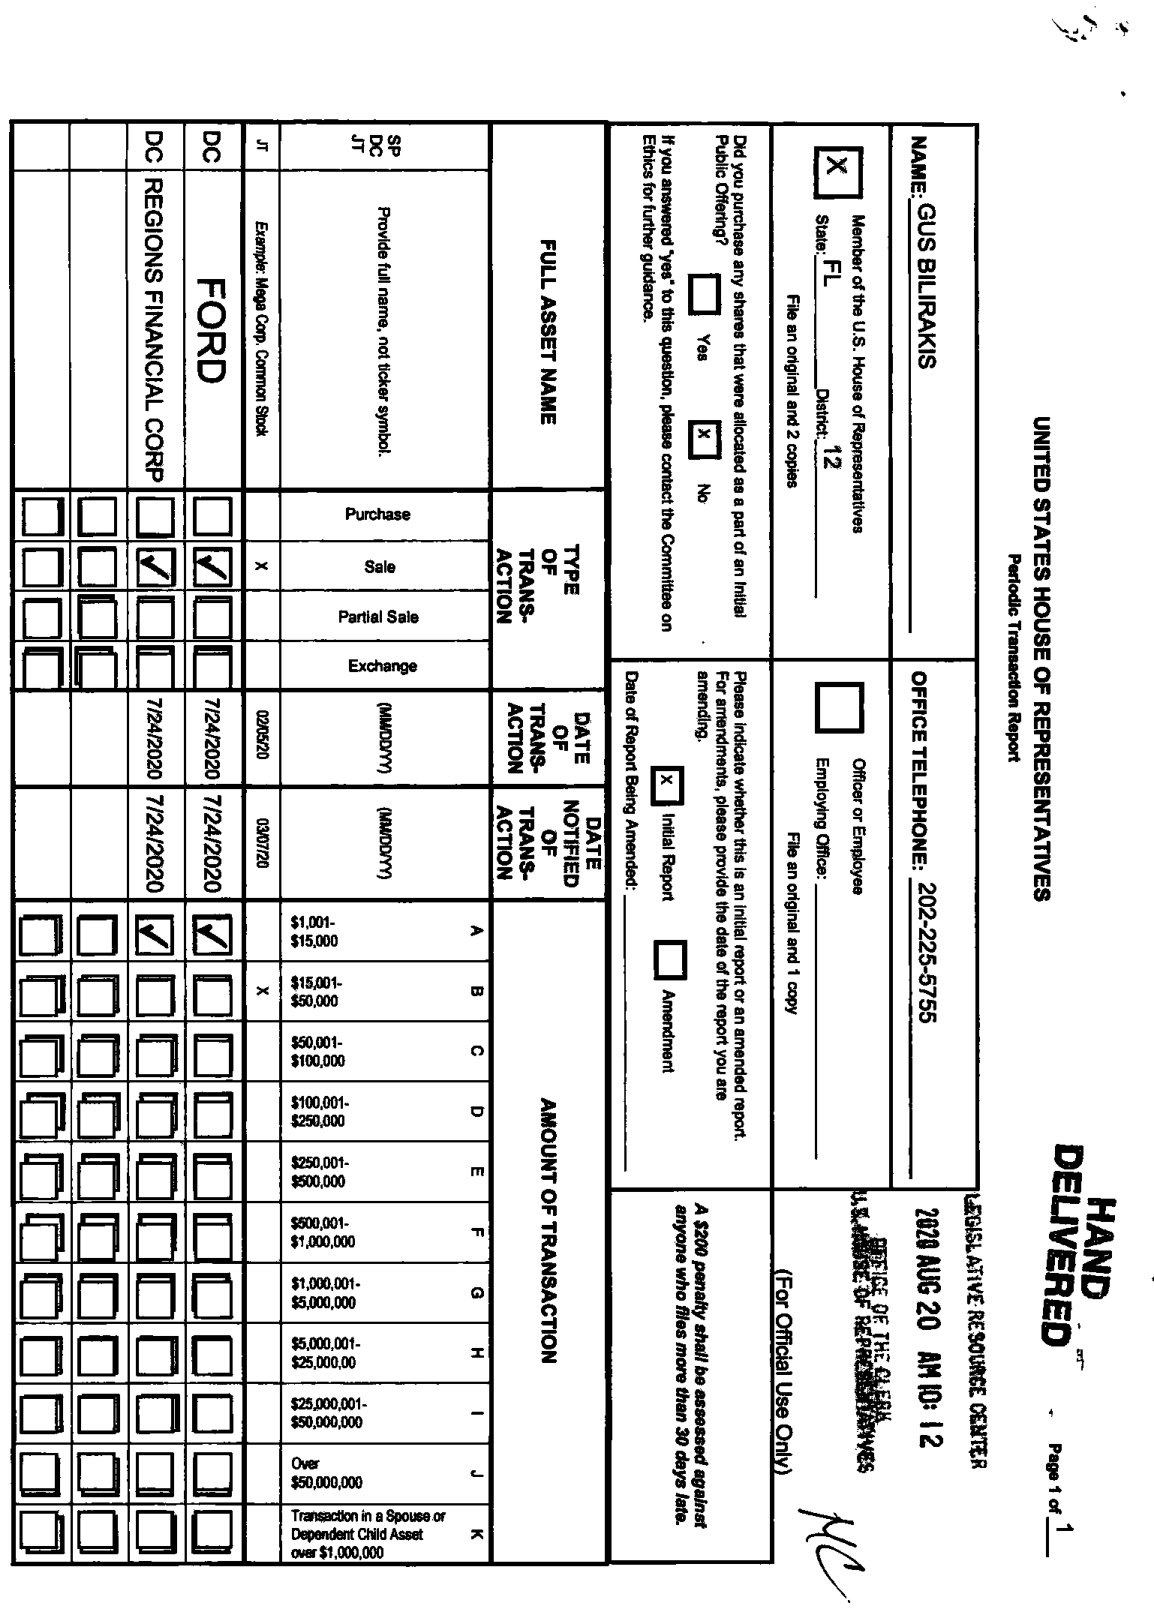
\includegraphics[height=31mm]{slides/scan_full_couche.png}}\\[1mm]
      {\footnotesize\textbf{Tapé, couché}}\\[0.3mm]
      {\scriptsize tourné à 90° --- lu quand même}
    \end{column}
    \begin{column}{0.37\textwidth}\centering
      \fcolorbox{black!30}{white}{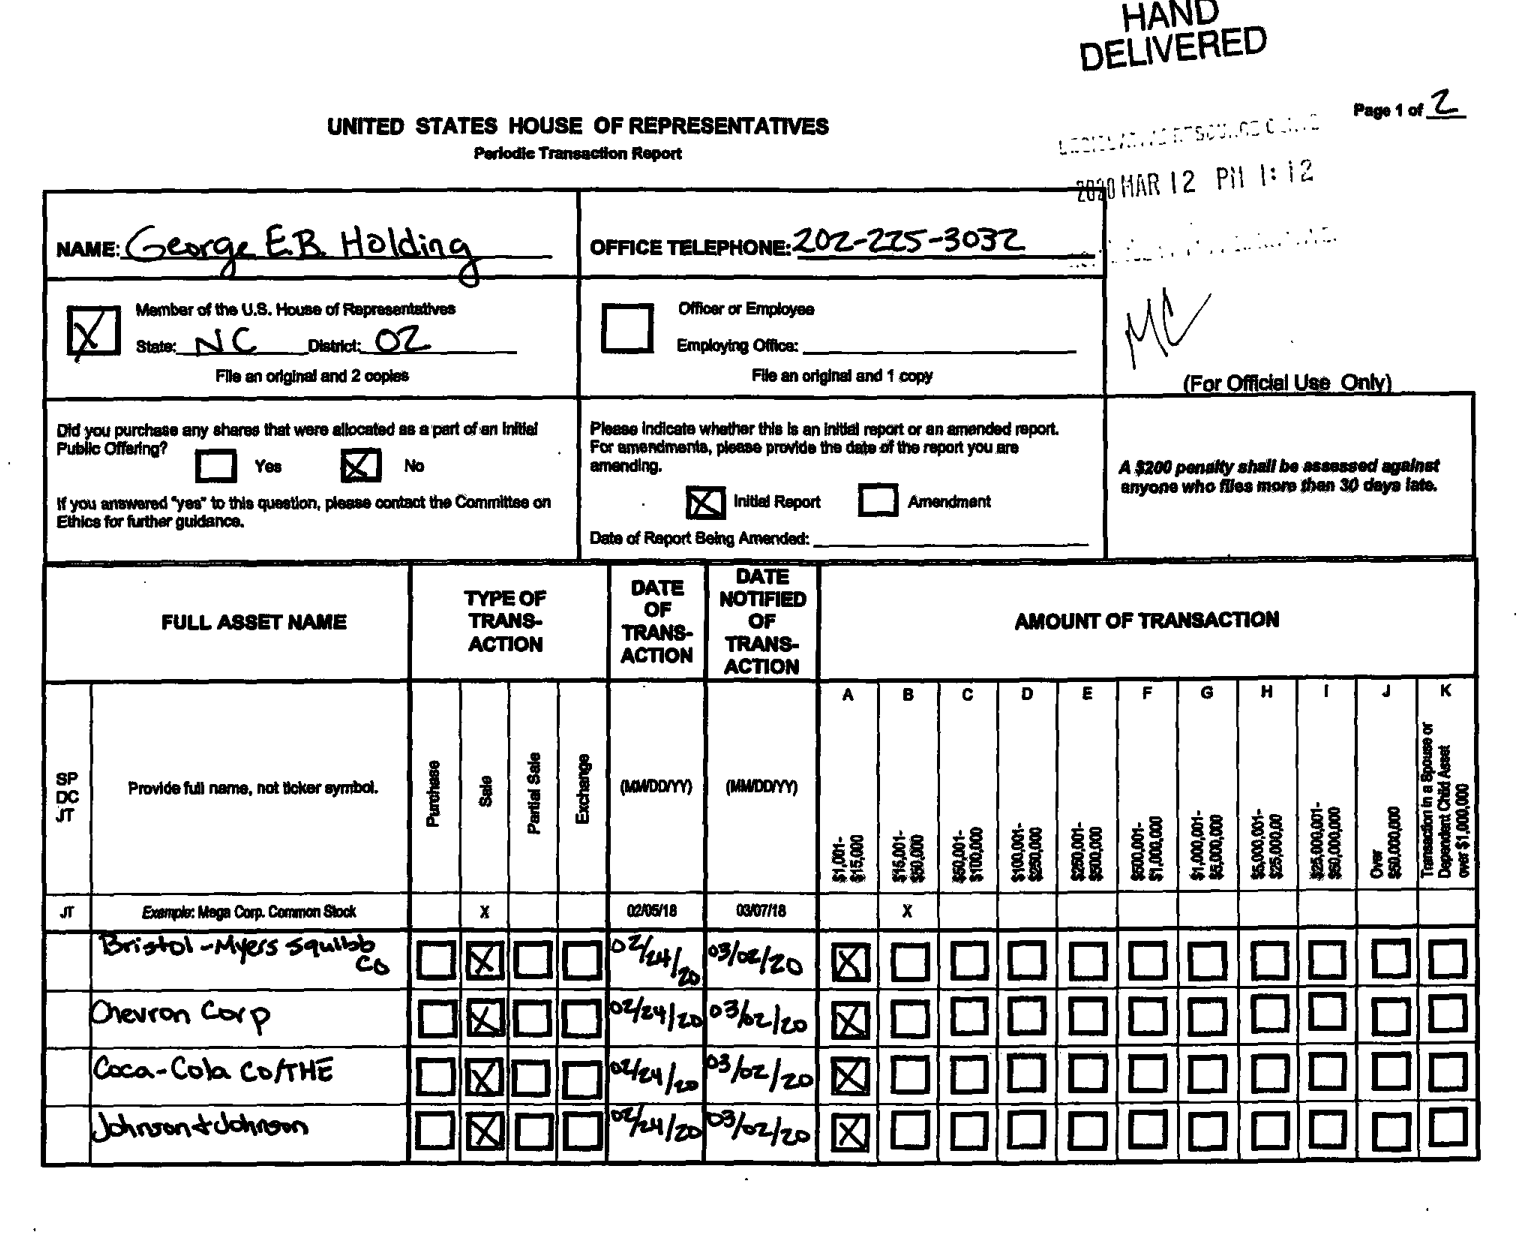
\includegraphics[height=31mm]{slides/scan_full_manuscrit.png}}\\[1mm]
      {\footnotesize\textbf{Manuscrit}}\\[0.3mm]
      {\scriptsize à la main, cursif --- \textbf{le vrai point dur}}
    \end{column}
  \end{columns}
  \vspace{2.5mm}
  \badgel{hocr}{775 scans manuscrits sur les 2\,424 scans Chambre recensés}\quad
  {\scriptsize\color{black!60} le papier existe aussi au Sénat, en faible volume ---
   il faudra une \textbf{politique} pour le manuscrit : \emph{tranchée à l'Étape 2}}
\end{frame}

% ── 1.5 · Les deux dates (S9 allégée) ──
\begin{frame}{Deux dates par transaction --- seule la date de dépôt est fiable : c'est elle le signal}
  \centering
  \vspace{1mm}
  \begin{columns}[T]
    \begin{column}{0.49\textwidth}\centering
      \colorbox{okgreen}{\parbox{0.94\linewidth}{\centering\vspace{0.4mm}{\color{white}\textbf{Date de DÉPÔT} \scriptsize(divulgation)}\vspace{0.4mm}}}\\[1.5mm]
      {\footnotesize \textbf{toujours une métadonnée} --- jamais lue dans le document,
       jamais OCRisée ; \textbf{fiable} → c'est la date \textbf{signal}}\\[1mm]
      {\scriptsize\color{black!60} délai médian de divulgation :
       \textbf{27 j} Chambre · \textbf{24 j} Sénat}
    \end{column}
    \begin{column}{0.49\textwidth}\centering
      \colorbox{warnorange}{\parbox{0.94\linewidth}{\centering\vspace{0.4mm}{\color{white}\textbf{Date de TRANSACTION}}\vspace{0.4mm}}}\\[1.5mm]
      {\footnotesize \textbf{lue dans le document} (texte ou OCR) ; la \textbf{seule
       risquée} → garde-fous $+$ flag, \textbf{jamais inventée}}\\[1mm]
      {\scriptsize\color{black!60} même schéma sur les 4 voies : le dépôt vient de
       l'index/du listing, la transaction du document}
    \end{column}
  \end{columns}
  \vspace{4mm}
  \choixbox{le signal est daté à la \textbf{date de dépôt} (divulgation), jamais à la
   date du trade : c'est ce qu'un investisseur réel aurait su, quand il l'aurait su
   (\textbf{anti-look-ahead}) --- et toute date de transaction douteuse est
   \textbf{flaguée, jamais réécrite au hasard}.}\\[2mm]
  {\scriptsize\color{black!55} garde-fou : une date de transaction hors de la fenêtre de
   plausibilité $[\text{dépôt}-90\,\text{j},\ +10\,\text{j}]$ → année recalée ou ligne
   flaguée}
\end{frame}

% ── 1.6 · Le corpus, concentré et papier (S10, McCaul corrigé) ── (ferme l'étape)
\begin{frame}{169\,000 transactions --- dont $\sim$40\,\% viennent de deux élus, exclusivement sur papier}
  \centering
  {\footnotesize \textbf{169\,000 transactions uniques} (2014--2026) --- ce que les
   étapes 2--3 vont extraire --- en quatre sous-corpus :}\\[1.2mm]
  \begin{tikzpicture}
    \draw[fill=helec, draw=none] (0,0) rectangle (4.176,0.5);
    \draw[fill=hocr, draw=none] (4.176,0) rectangle (10.8,0.5);
    \draw[fill=selec, draw=none] (10.8,0) rectangle (11.724,0.5);
    \draw[fill=socr, draw=none] (11.724,0) rectangle (12.0,0.5);
    \node[font=\scriptsize, color=white] at (2.09,0.25) {\textbf{Chambre élec.\ 34,8\,\%}};
    \node[font=\scriptsize, color=black!75] at (7.5,0.25) {\textbf{Chambre OCR 55,2\,\%}};
    \node[font=\tiny, color=white] at (11.26,0.25) {\textbf{7,7}};
    \node[font=\tiny, color=black!75, above=1mm of {(11.86,0.5)}] {Sénat OCR 2,4\,\%};
  \end{tikzpicture}\\[2mm]
  \begin{columns}[T]
    \begin{column}{0.55\textwidth}\centering
      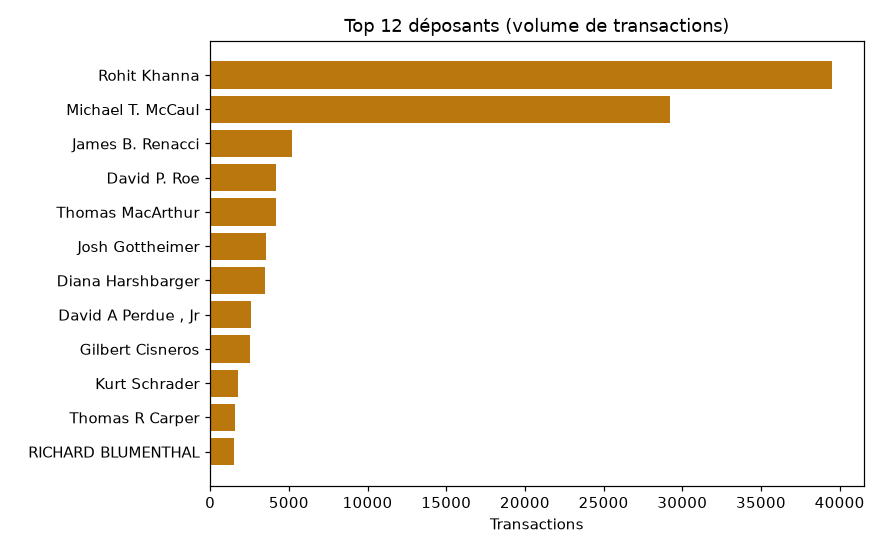
\includegraphics[width=0.74\linewidth]{quality/top_deposants.png}
    \end{column}
    \begin{column}{0.43\textwidth}
      \colorbox{warnorange!12}{\parbox{0.96\linewidth}{\footnotesize\vspace{0.5mm}
        \textbf{\textcolor{warnorange}{très concentré}} --- Khanna (\textbf{41\,080} txns)
        et McCaul (\textbf{27\,123}) pèsent à eux deux \textbf{$\sim$40\,\%} du corpus,
        et déclarent \textbf{exclusivement sur papier} (100\,\% OCR)\vspace{0.5mm}}}\\[1.5mm]
      {\footnotesize le papier n'est pas un détail : c'est \textbf{la majorité du corpus}
       (55,2\,\% rien que pour les scans Chambre)}
    \end{column}
  \end{columns}
  \vspace{1.5mm}
  \repband{2 guichets publics · 4 formats · 8\,252 PTR --- une matière majoritairement papier.}
\end{frame}

\section{Étape 2 · Le pipeline}
% ── intercalaire Étape 2 ──
\begin{frame}[plain]
  \centering
  \vspace{14mm}
  {\Large\bfseries\color{black!80} Étape 2 --- Le pipeline}\\[8mm]
  \begin{tikzpicture}[scale=1.0, every node/.style={transform shape}]
\node[rectangle, rounded corners=2.5pt, draw=okgreen, fill=okgreen!10, line width=0.8pt, text width=2.35cm, minimum height=1.05cm, align=center, font=\scriptsize] (b1) at (1.325,0) {\color{okgreen}\checkmark~\textbf{1 · \mbox{Donnée brute}}};
\draw[arr] (2.65,0) -- (3.07,0);
\node[rectangle, rounded corners=2.5pt, draw=grisC, fill=grisC, line width=0.8pt, text width=2.35cm, minimum height=1.05cm, align=center, font=\scriptsize] (b2) at (4.395,0) {\color{white}\textbf{2 · Pipeline}};
\draw[arr] (5.72,0) -- (6.14,0);
\node[rectangle, rounded corners=2.5pt, draw=dataC, fill=dataC!10, line width=0.8pt, text width=2.35cm, minimum height=1.05cm, align=center, font=\scriptsize] (b3) at (7.465,0) {\color{dataC}\textbf{3 · Enrichir}};
\draw[arr] (8.79,0) -- (9.209999999999999,0);
\node[rectangle, rounded corners=2.5pt, draw=alertred, fill=alertred!10, line width=1.3pt, text width=2.75cm, minimum height=1.05cm, align=center, font=\scriptsize] (b4) at (10.735,0) {\color{alertred}\textbf{4 · \mbox{VÉRIFICATION}}};
\draw[arr] (12.259999999999998,0) -- (12.679999999999998,0);
\node[rectangle, rounded corners=2.5pt, draw=okgreen, fill=okgreen!10, line width=0.8pt, text width=2.35cm, minimum height=1.05cm, align=center, font=\scriptsize] (b5) at (14.004999999999999,0) {\color{okgreen}\textbf{5 · Livrable}};
\end{tikzpicture}\\[9mm]
  {\normalsize\itshape\color{black!55} Comment passe-t-on de $\sim$10\,000 documents
   hétérogènes à une seule table ?}
\end{frame}

% ── 2.1 · Le flux (S11 conservée, allégée) ──
\begin{frame}{Le flux de bout en bout tient en une image}
  \centering
  \resizebox{!}{0.86\textheight}{%
  \begin{tikzpicture}[node distance=3mm]
    % ---- bande 1 : Acquisition + Tri ----
    \node[step=dataC, text width=6.2cm] (acqH) at (-3.7,0)
      {\textbf{\color{helec}Chambre} --- \emph{House Clerk} → index annuel → PDF};
    \node[step=dataC, text width=6.2cm] (acqS) at (3.7,0)
      {\textbf{\color{selec}Sénat} --- \emph{eFD} → liste des dépôts (HTML ou papier)};
    \node[step=helec, text width=2.9cm] (hpdf) at (-5.5,-1.35) {\textbf{PDF lisible}\\couche texte présente};
    \node[step=helec, text width=2.9cm] (hscan) at (-2.0,-1.35) {\textbf{scan tapé}\\image, souvent couchée};
    \node[step=selec, text width=2.9cm] (shtml) at (2.0,-1.35) {\textbf{page HTML}\\déclaration eFD};
    \node[step=selec, text width=2.9cm] (sgif) at (5.5,-1.35) {\textbf{image papier}\\souvent couchée};
    \node[step=alertred, text width=2.9cm, font=\tiny] (hC) at (-2.0,-2.5)
      {scan \textbf{manuscrit} → écarté (règle rejouable)};
    \node[font=\tiny\bfseries, text=gray!60, rotate=90] at (-7.6,0) {Acquisition};
    \node[font=\tiny\bfseries, text=gray!60, rotate=90] at (-7.6,-1.4) {Tri};
    \draw[arr] (acqH) -- (hpdf); \draw[arr] (acqH) -- (hscan);
    \draw[arr] (acqS) -- (shtml); \draw[arr] (acqS) -- (sgif);
    \draw[arr] (hscan) -- (hC);
    % ---- bande 2 : Extraction ----
    \visible<2->{
    \node[step=helec, text width=2.9cm] (hpar) at (-5.5,-2.75)
      {\textbf{parsing déterministe}\\[0.5mm]{\normalsize\textbf{\color{helec}58\,728}}};
    \node[step=helec, text width=2.9cm] (hvis) at (-2.0,-3.65)
      {\textbf{OCR Claude Vision} redressée, lue en JSON\\[0.5mm]{\normalsize\textbf{\color{helec}93\,261}}};
    \node[step=selec, text width=2.9cm] (spar) at (2.0,-2.75)
      {\textbf{lecture des tableaux}\\[0.5mm]{\normalsize\textbf{\color{selec}13\,026}}};
    \node[step=selec, text width=2.9cm] (svis) at (5.5,-2.75)
      {\textbf{OCR Claude Vision}\\sans redressement\\[0.5mm]{\normalsize\textbf{\color{selec}3\,985}}};
    \node[font=\tiny\bfseries, text=gray!60, rotate=90] at (-7.6,-3.2) {Extraction};
    \draw[arr] (hpdf) -- (hpar); \draw[arr] (hscan) -- (hvis);
    \draw[arr] (shtml) -- (spar); \draw[arr] (sgif) -- (svis);}
    % ---- bande 3 : Tronc commun ----
    \visible<3->{
    \node[bande=grisC, text width=13.6cm] (conv) at (0,-4.85)
      {\textbf{lignes normalisées} --- déclarant, dates (trade + divulgation), actif,
       opération, fourchette, détenteur};
    \node[bande=grisC, text width=13.6cm] (ident) at (0,-5.75)
      {\textbf{identité} --- nom libre → identifiant officiel de l'élu (+ parti,
       commissions) \emph{(détail 4 slides plus loin)}};
    \node[bande=grisC, text width=13.6cm] (enr) at (0,-6.65)
      {\textbf{enrichissement} --- ticker · secteur → ETF · montant → \emph{milieu de
       fourchette} \emph{(détail : Étape 3)}};
    \node[font=\tiny\bfseries, text=gray!60, rotate=90] at (-7.6,-5.75) {Tronc commun};
    \draw[arr] (hpar.south) -- (conv.north -| hpar.south);
    \draw[arr] (hvis.south) -- (conv.north -| hvis.south);
    \draw[arr] (spar.south) -- (conv.north -| spar.south);
    \draw[arr] (svis.south) -- (conv.north -| svis.south);
    \draw[arr] (conv) -- (ident); \draw[arr] (ident) -- (enr);}
    % ---- bande 4 : Livraison ----
    \visible<4->{
    \node[bande=dataC, fill=dataC!14, text width=13.6cm] (fin) at (0,-7.65)
      {\textbf{TABLE DU CORPUS} --- \textbf{169\,000 uniques} (170\,920 lignes) ·
       28 colonnes};
    \node[bande=dataC, fill=dataC!14, text width=13.6cm] (clean) at (0,-8.65)
      {\textbf{TABLE DE RECHERCHE} --- \textbf{134\,464 × 36} · entonnoir
       \emph{(Étape 5)}};
    \node[font=\tiny\bfseries, text=gray!60, rotate=90] at (-7.6,-8.15) {Livraison};
    \draw[arr] (enr) -- (fin);
    \draw[arr] (fin) -- (clean);}
  \end{tikzpicture}}
\end{frame}

% ── 2.2 · Les voies électroniques (fusion S13+S5b) ──
\begin{frame}{Les deux voies électroniques : du parsing déterministe de bout en bout}
  \begin{columns}[T]
    \begin{column}{0.52\textwidth}\centering
      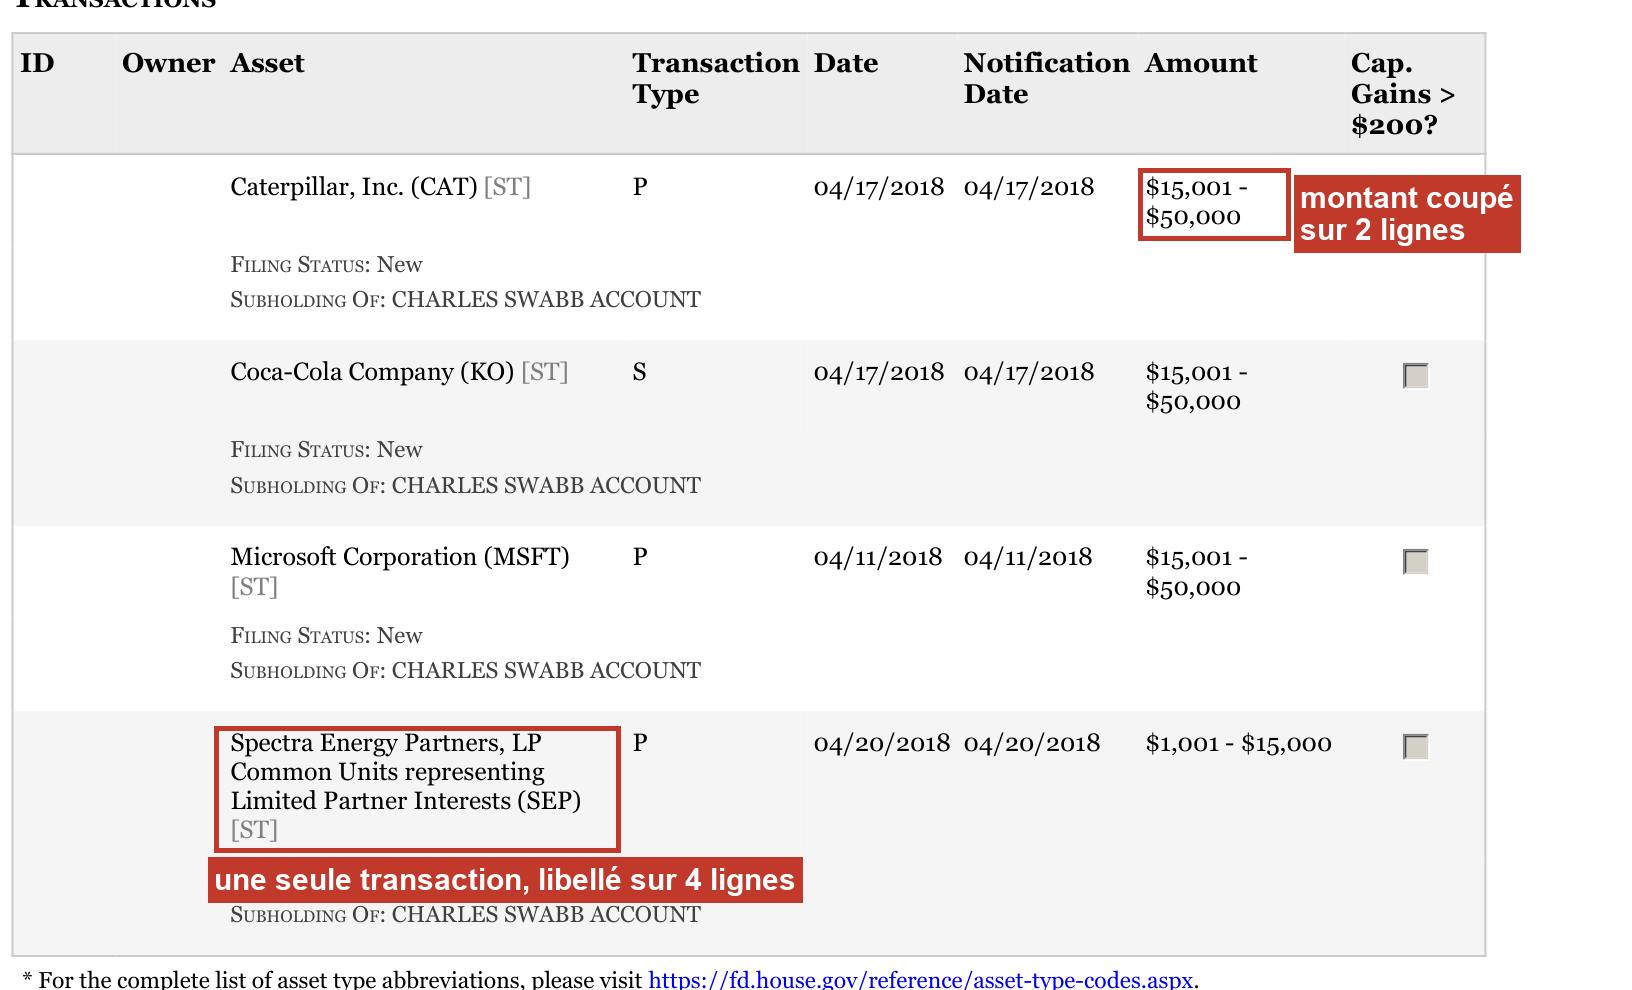
\includegraphics[width=\linewidth,height=0.46\textheight,keepaspectratio]{slides/fig_ptr_multiligne.png}\\[0.5mm]
      {\scriptsize\color{black!60} extrait réel --- le montant déborde sur la ligne
       suivante, le libellé court sur 4 lignes : \textbf{un parseur naïf raterait la
       moitié} → on \textbf{reconstruit} chaque transaction avant de la lire}
    \end{column}
    \begin{column}{0.44\textwidth}
      \badge{helec}{Chambre --- 58\,728 transactions}\\[1.2mm]
      {\footnotesize recoller les lignes coupées → repérer la signature (opération +
       2 dates + fourchette) → rattacher l'actif}\\[2mm]
      \badge{selec}{Sénat --- 13\,026 transactions}\\[1.2mm]
      {\footnotesize liste des dépôts → page HTML par dépôt → lecture des tableaux
       (gabarit stable sur 13 ans)}\\[2mm]
      {\scriptsize\color{black!60} pour le texte, \textbf{pas d'IA} : du code
       déterministe, rejouable à l'identique · zéro échec silencieux (les dépôts sans
       transaction sont tous consignés)}
    \end{column}
  \end{columns}
  \vspace{1.5mm}
  \choixbox{la Chambre a \textbf{deux gabarits} de formulaire (l'ancien sans code type
   d'actif, le moderne avec \co{[ST]}, apparu vers 2018) --- \textbf{routés document par
   document}, jamais par année fixe.}
\end{frame}

% ── 2.3 · Scans Chambre : écarté car mesurable (S14 allégée) ──
\begin{frame}{Les scans Chambre : Vision lit tout --- le manuscrit est écarté par une règle mesurée}
  \centering
  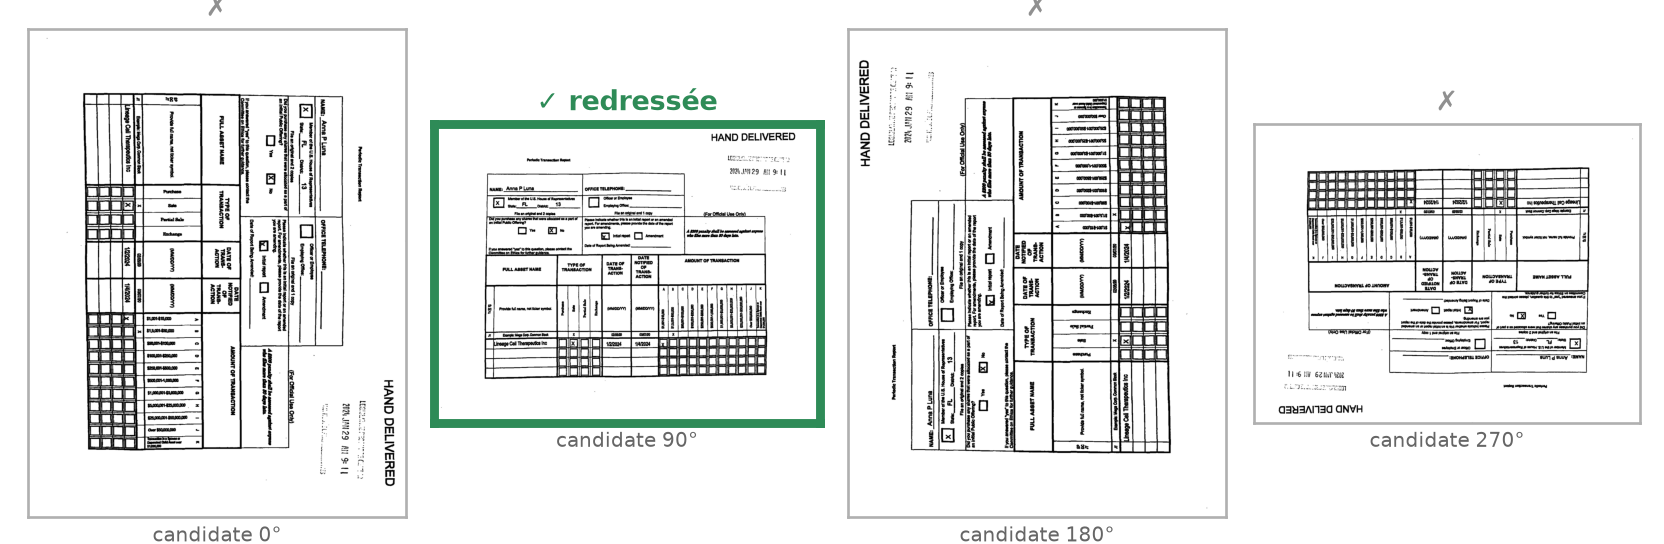
\includegraphics[width=0.50\textwidth]{slides/fig_deskew_rotations.png}
  \vspace{1mm}
  \begin{columns}[T]
    \begin{column}{0.44\textwidth}\footnotesize
      · l'\textbf{OCR par IA} (Claude Vision) lit le tapé, même tourné à 90°\\[1mm]
      · \badgel{hocr}{93\,261 transactions extraites des scans}\\[1mm]
      · {\scriptsize\color{black!60} très concentrées : les gros déposants
        « 100\,\% papier » de l'Étape 1}
    \end{column}
    \begin{column}{0.54\textwidth}\footnotesize
      \colorbox{black!6}{\parbox{0.97\linewidth}{\scriptsize
        \textbf{la mesure} --- \textbf{Quiver Quantitative} (fournisseur commercial des
        mêmes données, notre mètre externe --- détail Étape 4), \emph{même sans exiger
        la date}, ne corrobore que \textbf{12,9\,\%} du manuscrit, contre \textbf{88\,\%}
        du tapé droit}}\\[1.5mm]
      \badge{alertred}{582 PTR manuscrits écartés --- 7,1 \% de l'index}
    \end{column}
  \end{columns}
  \vspace{2mm}
  \choixbox{\textbf{on ne met en table que ce qu'on sait lire} : les 582 PTR manuscrits
   sont écartés par une \textbf{règle écrite et rejouable}, avec exceptions explicites
   --- pas de lectures douteuses injectées dans la donnée.}
\end{frame}

% ── 2.4 · Papier Sénat : gardé car non mesurable (S15 allégée, miroir) ──
\begin{frame}{Le papier Sénat : gardé --- faute de mètre externe pour le mesurer}
  \begin{columns}[c]
    \begin{column}{0.30\textwidth}\centering
      \fcolorbox{black!30}{white}{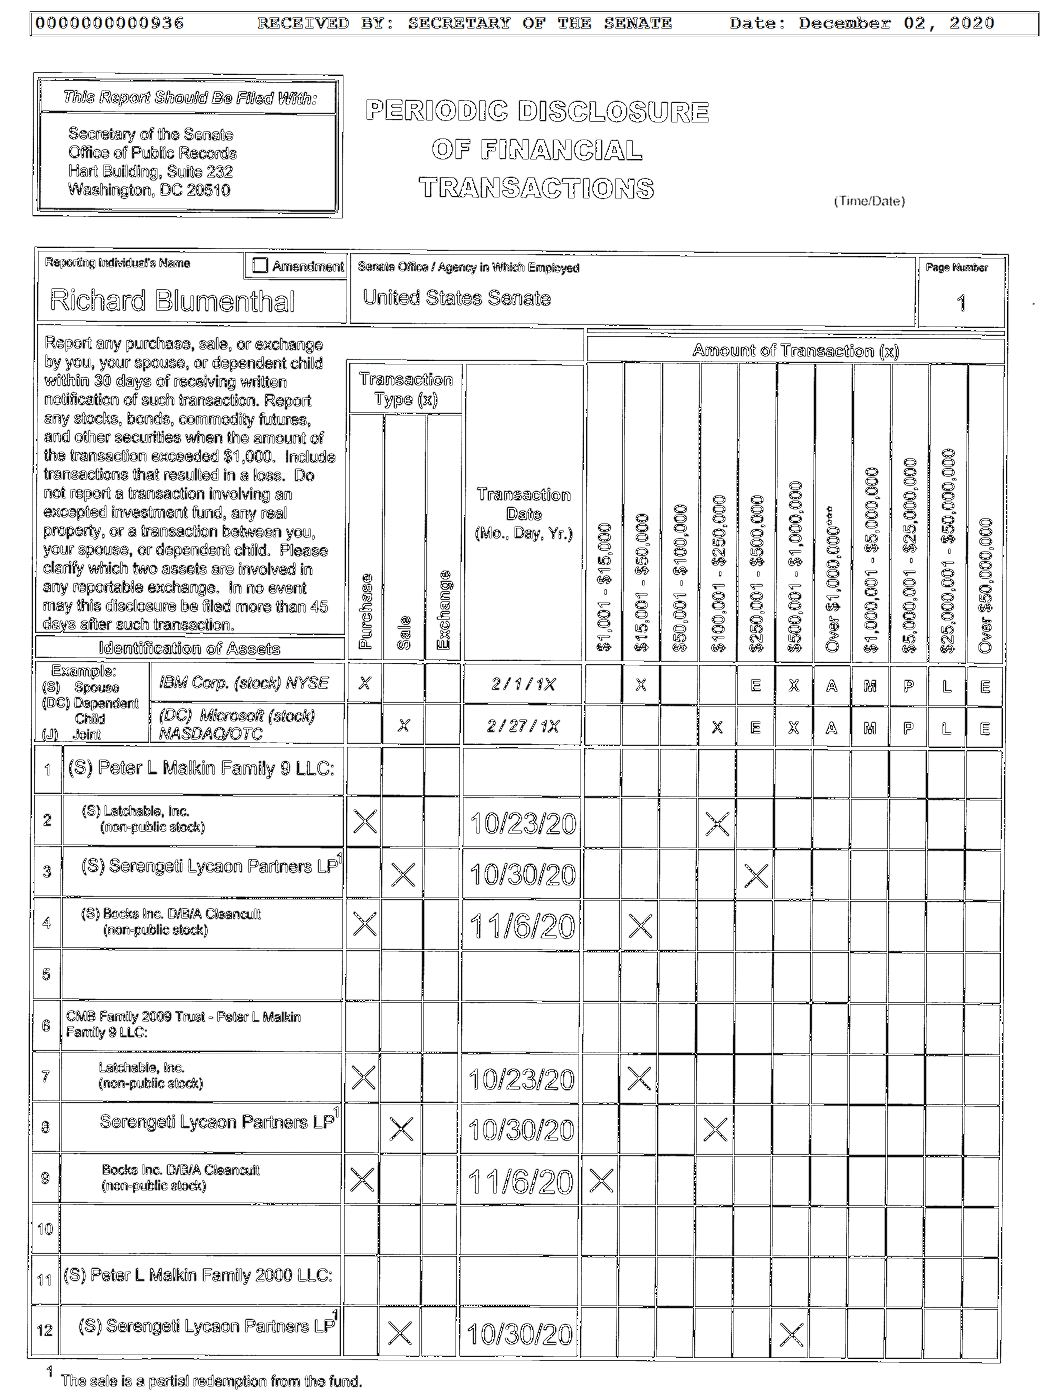
\includegraphics[height=42mm]{slides/senat_papier_droit.png}}\\[0.8mm]
      {\scriptsize\color{black!60} le formulaire papier Sénat}
    \end{column}
    \begin{column}{0.66\textwidth}
      {\scriptsize ce que rend l'OCR, transaction par transaction (extrait réel --- John Boozman) :}\\[1mm]
      {\footnotesize
      \begin{tabular}{@{}ll@{}}
        \toprule
        actif · opération & Apple Computer Inc · \textbf{Sale} \\
        date du trade · fourchette & 2022-03-14 · code A (1\,001--15\,000 \$) \\
        \bottomrule
      \end{tabular}}\\[2.5mm]
      \badgel{socr}{3\,985 transactions --- 14 déposants --- 2,4 \% du corpus}\\[1.5mm]
      {\footnotesize même moteur de lecture que la Chambre --- mais \textbf{politique
       inverse} : Quiver est \textbf{aveugle au papier du Sénat} → aucune mesure
       d'exclusion possible → on \textbf{garde}, sous garde-fous internes, et on
       l'écrit}\\[1mm]
      {\scriptsize\color{black!60} couverture ticker plus basse sur cette voie =
       \textbf{composition, pas défaut} : Blumenthal porte 38,7\,\% de la voie,
       massivement du non-coté}
    \end{column}
  \end{columns}
  \vspace{1.5mm}
  \choixbox{on n'écarte que ce qu'on a pu \textbf{mesurer} --- l'asymétrie
   Chambre/Sénat (écarté ici, gardé là) est \textbf{documentée, pas cachée} ; le risque
   est borné (2,4\,\% du corpus).}
\end{frame}

% ── 2.5 · Identité 100 % (S12 allégée) ── (ferme l'étape)
\begin{frame}{Chaque ligne est rattachée à un élu officiel : identité 100\,\%}
  \begin{columns}[T]
    \begin{column}{0.58\textwidth}
      {\footnotesize un même élu signe « Hon.\ Earl L.\ Carter », « Buddy Carter »,
       « N.\ Pelosi »… → on relie ce \textbf{nom libre} à un \textbf{identifiant unique},
       par une cascade d'essais :}\\[2mm]
      \centering
      \begin{tikzpicture}[node distance=2.6mm]
        \node[step=grisC, text width=6.6cm] (n) {\textbf{nom libre du formulaire}};
        \node[step=helec, text width=6.6cm, below=of n] (c1)
          {1. \textbf{override manuel} --- un seul cas par chambre};
        \node[step=helec, text width=6.6cm, below=of c1] (c2)
          {2. \textbf{correspondance exacte} --- accents, titres (\emph{Hon., Dr.}),
           suffixes, diminutifs (\emph{William → Bill})};
        \node[step=helec, text width=6.6cm, below=of c2] (c3)
          {3. \textbf{repli nom de famille} (s'il ne désigne qu'un élu)};
        \node[step=okgreen, text width=6.6cm, below=of c3] (r)
          {identifiant officiel (\co{bioguide}) → \textbf{parti + commissions} joints};
        \draw[arr] (n) -- (c1); \draw[arr] (c1) -- (c2);
        \draw[arr] (c2) -- (c3); \draw[arr] (c3) -- (r);
      \end{tikzpicture}
    \end{column}
    \begin{column}{0.40\textwidth}
      \badge{okgreen}{100\,\% des lignes rattachées}\\[1mm]
      {\footnotesize \textbf{367} membres Chambre · \textbf{78} Sénat}\\[2mm]
      {\scriptsize\color{black!60} le \emph{bioguide} = l'identifiant officiel unique
       d'un élu au Congrès (annuaire public \emph{congress-legislators})}\\[3mm]
      \choixbox{les fichiers extraits sont \textbf{figés} ; toute réparation (coquille,
       identifiant manquant) est appliquée \textbf{à la lecture}, jamais en réécrivant
       la source --- l'audit reste possible à l'octet près.}
    \end{column}
  \end{columns}
  \vspace{1.5mm}
  \centering
  \repband{58\,728 + 93\,261 + 13\,026 + 3\,985 = \textbf{169\,000} transactions
   extraites, \textbf{100\,\%} identifiées.}
\end{frame}

\section{Étape 3 · Enrichir}
% ── intercalaire Étape 3 ──
\begin{frame}[plain]
  \centering
  \vspace{14mm}
  {\Large\bfseries\color{black!80} Étape 3 --- Enrichir}\\[8mm]
  \begin{tikzpicture}[scale=1.0, every node/.style={transform shape}]
\node[rectangle, rounded corners=2.5pt, draw=okgreen, fill=okgreen!10, line width=0.8pt, text width=2.35cm, minimum height=1.05cm, align=center, font=\scriptsize] (b1) at (1.325,0) {\color{okgreen}\checkmark~\textbf{1 · \mbox{Donnée brute}}};
\draw[arr] (2.65,0) -- (3.07,0);
\node[rectangle, rounded corners=2.5pt, draw=okgreen, fill=okgreen!10, line width=0.8pt, text width=2.35cm, minimum height=1.05cm, align=center, font=\scriptsize] (b2) at (4.395,0) {\color{okgreen}\checkmark~\textbf{2 · Pipeline}};
\draw[arr] (5.72,0) -- (6.14,0);
\node[rectangle, rounded corners=2.5pt, draw=dataC, fill=dataC, line width=0.8pt, text width=2.35cm, minimum height=1.05cm, align=center, font=\scriptsize] (b3) at (7.465,0) {\color{white}\textbf{3 · Enrichir}};
\draw[arr] (8.79,0) -- (9.209999999999999,0);
\node[rectangle, rounded corners=2.5pt, draw=alertred, fill=alertred!10, line width=1.3pt, text width=2.75cm, minimum height=1.05cm, align=center, font=\scriptsize] (b4) at (10.735,0) {\color{alertred}\textbf{4 · \mbox{VÉRIFICATION}}};
\draw[arr] (12.259999999999998,0) -- (12.679999999999998,0);
\node[rectangle, rounded corners=2.5pt, draw=okgreen, fill=okgreen!10, line width=0.8pt, text width=2.35cm, minimum height=1.05cm, align=center, font=\scriptsize] (b5) at (14.004999999999999,0) {\color{okgreen}\textbf{5 · Livrable}};
\end{tikzpicture}\\[9mm]
  {\normalsize\itshape\color{black!55} Que faut-il ajouter pour qu'un backtest puisse s'en servir ?}
\end{frame}

% ── 3.1 · Ticker + secteur (fusion S16a+S16b) ──
\begin{frame}{Chaque transaction reçoit un ticker et un secteur --- par deux cascades tracées}
  \begin{columns}[c]
    \begin{column}{0.56\textwidth}\footnotesize
      \begin{tikzpicture}[node distance=2.6mm]
        \node[bande=helec, text width=6.8cm] (t1) {1. \textbf{explicite} --- déjà imprimé dans la source (l'électronique)};
        \node[bande=helec, text width=6.8cm, below=of t1] (t2) {2. \textbf{dictionnaire} --- le nom vu ailleurs dans le corpus (le papier)};
        \node[bande=helec, text width=6.8cm, below=of t2] (t3) {3. \textbf{LLM} contraint « actions seulement »};
        \node[bande=okgreen, text width=6.8cm, below=of t3] (t4) {4. \textbf{récupération} validée par double preuve --- \textbf{2\,540} lignes retrouvent leur symbole};
        \draw[arr] (t1) -- (t2); \draw[arr] (t2) -- (t3); \draw[arr] (t3) -- (t4);
      \end{tikzpicture}\\[1.5mm]
      {\scriptsize\color{black!60} même logique pour le \textbf{secteur} (11 secteurs
       GICS, la classification standard --- chacun adossé à son ETF sectoriel) :
       \textbf{79,8\,\%} Ch.\ · \textbf{70,4\,\%} Sén.}
    \end{column}
    \begin{column}{0.42\textwidth}\footnotesize
      \badge{helec}{ticker renseigné}\\[1mm]
      {\footnotesize \textbf{84,1\,\%} Chambre · \textbf{77,9\,\%} Sénat}\\[2.5mm]
      \colorbox{black!6}{\parbox{0.96\linewidth}{\scriptsize
        \textbf{couverture = remplissage, pas exactitude} --- les vides sont le
        \textbf{non-coté légitime} (munis, obligations, fonds privés),
        pas des défauts d'extraction}}\\[2.5mm]
      \choixbox{cascade \textbf{ordonnée et tracée}, du plus sûr au moins sûr --- chaque
       étage est enregistré ligne à ligne : jamais une devinette silencieuse.}
    \end{column}
  \end{columns}
\end{frame}

% ── 3.2 · L'empreinte (moitié S17) ──
\begin{frame}{Une transaction = 7 champs : l'empreinte dédoublonne sans jamais détruire}
  \begin{columns}[T]
    \begin{column}{0.55\textwidth}\footnotesize
      \textbf{l'empreinte d'une transaction --- 7 champs} :\\
      {\scriptsize \textbf{qui} (déclarant) · \textbf{quand} (date du trade) ·
       \textbf{quoi} (actif) · \textbf{sens} · \textbf{montant} (fourchette) ·
       \textbf{pour qui} (détenteur) · \textbf{chambre}}\\[2mm]
      {\scriptsize elle exclut \textbf{délibérément} :\\
       · le \textbf{ticker} --- ajouté après coup (Étape 3), sa présence rendrait
         l'empreinte instable\\
       · la \textbf{date de divulgation} --- un dépôt et son amendement portent le
         \emph{même} trade → une seule transaction}\\[2.5mm]
      \choixbox{dédup \textbf{non destructrice} : deux dépôts, même empreinte = un seul
       trade --- mais un \textbf{vrai lot répété} (même titre, plusieurs comptes) est
       \textbf{préservé} par un compteur d'occurrence. Jamais de dédoublonnage aveugle.}
    \end{column}
    \begin{column}{0.43\textwidth}
      \centering
      \begin{tikzpicture}[node distance=3mm]
        \node[bande=grisC, text width=4.9cm] (a) {\textbf{170\,920} lignes brutes};
        \node[bande=grisC, text width=4.9cm, below=of a] (b) {re-divulgations dédoublonnées \textbf{−1\,920}};
        \node[bande=dataC, fill=dataC!14, text width=4.9cm, below=of b] (c)
          {\textbf{169\,000 transactions uniques}};
        \draw[arr] (a) -- (b); \draw[arr] (b) -- (c);
      \end{tikzpicture}
    \end{column}
  \end{columns}
\end{frame}

% ── 3.3 · Le contrat 12 champs (moitié S17 + convention montant) ── (ferme l'étape)
\begin{frame}{Le contrat de la table corpus : 12 champs garantis, montant = milieu de fourchette}
  \centering
  \colorbox{helec}{\parbox{0.9\textwidth}{\footnotesize\color{white}\centering\vspace{0.6mm}
    \textbf{12 champs garantis} sur chaque ligne, pour les 2 chambres :\\
    déclarant · chambre · parti · commissions · date du trade · date de divulgation ·
    sens · montant · type d'actif · ticker · secteur · ETF\vspace{0.6mm}}}\\[3mm]
  \begin{columns}[T]
    \begin{column}{0.52\textwidth}\footnotesize
      \textbf{la convention de montant} :\\[1mm]
      {\scriptsize la loi ne donne qu'une \textbf{fourchette}
       (ex.\ 15\,001--50\,000~\$) --- on prend son \textbf{milieu exact} :
       32\,500\textbf{,5}~\$ (d'où les « ,5 » dans la table)}\\[2.5mm]
      \choixbox{une convention \textbf{unique et documentée} (le milieu de fourchette)
       plutôt qu'une fausse précision --- le montant est renseigné à 99,4\,\%.}
    \end{column}
    \begin{column}{0.44\textwidth}\footnotesize
      \textbf{la table du corpus} :\\[1mm]
      \badge{dataC}{169\,000 lignes × 28 colonnes}\\[1.5mm]
      {\scriptsize chaque ligne garde aussi sa \textbf{traçabilité} : le document
       source, l'empreinte, la voie d'extraction}
    \end{column}
  \end{columns}
  \vspace{3mm}
  \repband{169\,000 transactions uniques · 12 champs garantis · chaque enrichissement tracé.}
\end{frame}

\section{Étape 4 · Vérification}
% ── intercalaire Étape 4 ──
\begin{frame}[plain]
  \centering
  \vspace{14mm}
  {\Large\bfseries\color{black!80} Étape 4 --- Vérification}\\[8mm]
  \begin{tikzpicture}[scale=1.0, every node/.style={transform shape}]
\node[rectangle, rounded corners=2.5pt, draw=okgreen, fill=okgreen!10, line width=0.8pt, text width=2.35cm, minimum height=1.05cm, align=center, font=\scriptsize] (b1) at (1.325,0) {\color{okgreen}\checkmark~\textbf{1 · \mbox{Donnée brute}}};
\draw[arr] (2.65,0) -- (3.07,0);
\node[rectangle, rounded corners=2.5pt, draw=okgreen, fill=okgreen!10, line width=0.8pt, text width=2.35cm, minimum height=1.05cm, align=center, font=\scriptsize] (b2) at (4.395,0) {\color{okgreen}\checkmark~\textbf{2 · Pipeline}};
\draw[arr] (5.72,0) -- (6.14,0);
\node[rectangle, rounded corners=2.5pt, draw=okgreen, fill=okgreen!10, line width=0.8pt, text width=2.35cm, minimum height=1.05cm, align=center, font=\scriptsize] (b3) at (7.465,0) {\color{okgreen}\checkmark~\textbf{3 · Enrichir}};
\draw[arr] (8.79,0) -- (9.209999999999999,0);
\node[rectangle, rounded corners=2.5pt, draw=alertred, fill=alertred, line width=1.3pt, text width=2.75cm, minimum height=1.05cm, align=center, font=\scriptsize] (b4) at (10.735,0) {\color{white}\textbf{4 · \mbox{VÉRIFICATION}}};
\draw[arr] (12.259999999999998,0) -- (12.679999999999998,0);
\node[rectangle, rounded corners=2.5pt, draw=okgreen, fill=okgreen!10, line width=0.8pt, text width=2.35cm, minimum height=1.05cm, align=center, font=\scriptsize] (b5) at (14.004999999999999,0) {\color{okgreen}\textbf{5 · Livrable}};
\end{tikzpicture}\\[9mm]
  {\normalsize\itshape\color{black!55} Comment sait-on qu'on n'a \textbf{rien raté} ---
   ni \textbf{rien inventé} ?}
\end{frame}

% ── 4.1 · Les trois questions (S18 conservée, légendes précisées) ──
\begin{frame}{Vérifier, c'est répondre à trois questions}
  \centering
  \vspace{2mm}
  \begin{columns}[T]
    \begin{column}{0.32\textwidth}\centering
      \colorbox{helec!10}{\parbox[t][47mm][t]{\dimexpr\linewidth-8pt}{\vspace{1.5mm}\centering
        {\color{helec}\large\textbf{1 · Complétude}}\\[2mm]
        {\footnotesize « A-t-on couvert \textbf{tout} le périmètre ? »}\\[3mm]
        {\scriptsize on ouvre les \textbf{11 autres types} de dépôts
         et on mesure le trou}\\[2.5mm]
        {\color{helec}\Large\textbf{173}}\\[0.5mm]{\tiny actions résiduelles échappant au signal}}}
    \end{column}
    \begin{column}{0.32\textwidth}\centering
      \colorbox{okgreen!10}{\parbox[t][47mm][t]{\dimexpr\linewidth-8pt}{\vspace{1.5mm}\centering
        {\color{okgreen}\large\textbf{2 · Cohérence}}\\[2mm]
        {\footnotesize « Les flux se \textbf{recollent}-ils comptablement ? »}\\[3mm]
        {\scriptsize patrimoine d'entrée + nos transactions
         $\overset{?}{=}$ patrimoine de sortie}\\[2.5mm]
        {\color{okgreen}\Large\textbf{87,8\,\%}}\\[0.5mm]{\tiny des positions de sortie expliquées (Chambre)}}}
    \end{column}
    \begin{column}{0.32\textwidth}\centering
      \colorbox{dataC!10}{\parbox[t][47mm][t]{\dimexpr\linewidth-8pt}{\vspace{1.5mm}\centering
        {\color{dataC}\large\textbf{3 · Corroboration}}\\[2mm]
        {\footnotesize « Des \textbf{tiers indépendants} voient-ils la même chose ? »}\\[3mm]
        {\scriptsize Quiver + collectes indépendantes ---
         jamais réinjectés}\\[2.5mm]
        {\color{dataC}\Large\textbf{93,5\,\%}}\\[0.5mm]{\tiny des combinaisons du tiers retrouvées chez nous (Chambre)}}}
    \end{column}
  \end{columns}
  \vspace{4mm}
  {\footnotesize une seule question, en réalité --- \textbf{peut-on faire confiance à la table ?} ---
   posée \textbf{de l'intérieur} (1, 2) puis \textbf{de l'extérieur} (3)}
\end{frame}

% ── 4.2 · Complétude : les 11 autres types (fusion S19+S20) ──
\begin{frame}{Complétude : on ouvre les 11 autres types --- les transactions ne vivent que dans P, O, T}
  \badgel{helec!30}{Question 1 · Complétude}\\[0.5mm]
  \centering
  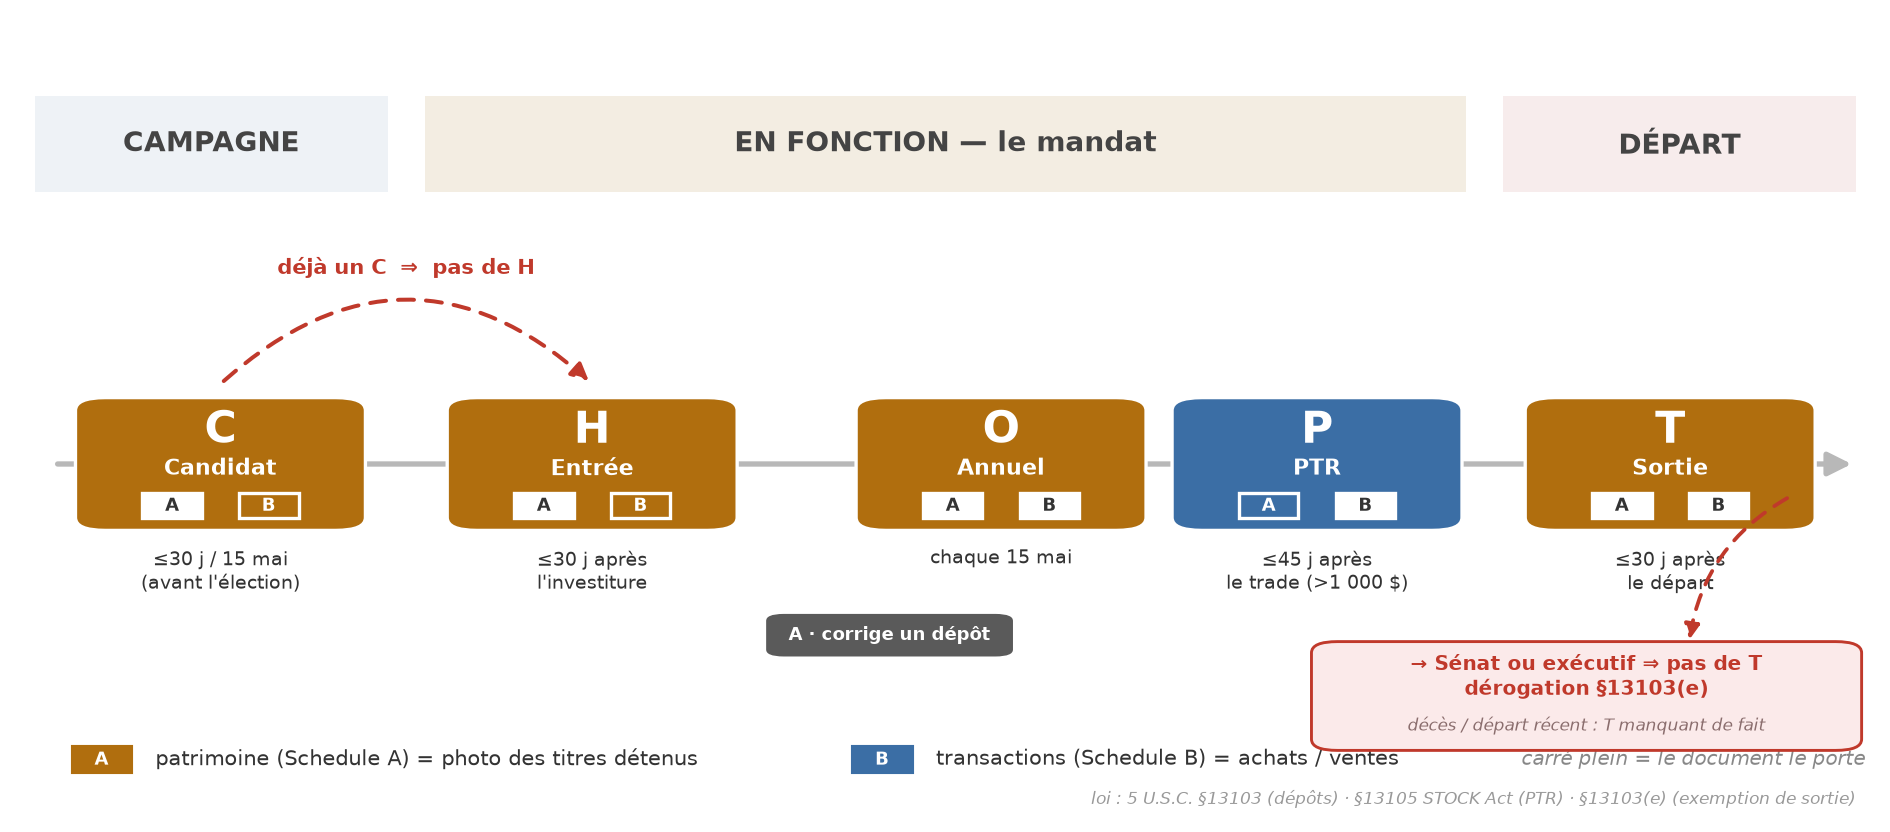
\includegraphics[width=0.72\textwidth,height=0.46\textheight,keepaspectratio]{slides/fig_house_loi_cycle.png}\\[0.8mm]
  {\footnotesize la vie déclarative d'un élu : chaque étape a son dépôt --- Schedule
   \textbf{A} = la \textbf{photo du patrimoine} · Schedule \textbf{B} = la \textbf{liste
   des transactions} ; hors PTR, les transactions ne vivent que dans l'annuel
   \textbf{O} (4\,625 dépôts, \textbf{31\,\%} avec transactions), la sortie \textbf{T}
   et leurs amendements --- \textbf{57\,259} lignes brutes au total (verdict slide
   suivante)}\\[0.5mm]
  {\scriptsize\color{black!60} les photos H/T serviront à la question 2 (Cohérence)}
\end{frame}

% ── 4.3 · Verdict complétude (essence S21 + Coh-5) ──
\begin{frame}{Verdict complétude : le hors-PTR est du patrimoine découvert trop tard --- le signal ne perd que 173 actions}
  \badgel{helec!30}{Question 1 · Complétude}\\[1mm]
  \begin{columns}[c]
    \begin{column}{0.46\textwidth}\centering
      \fcolorbox{black!25}{white}{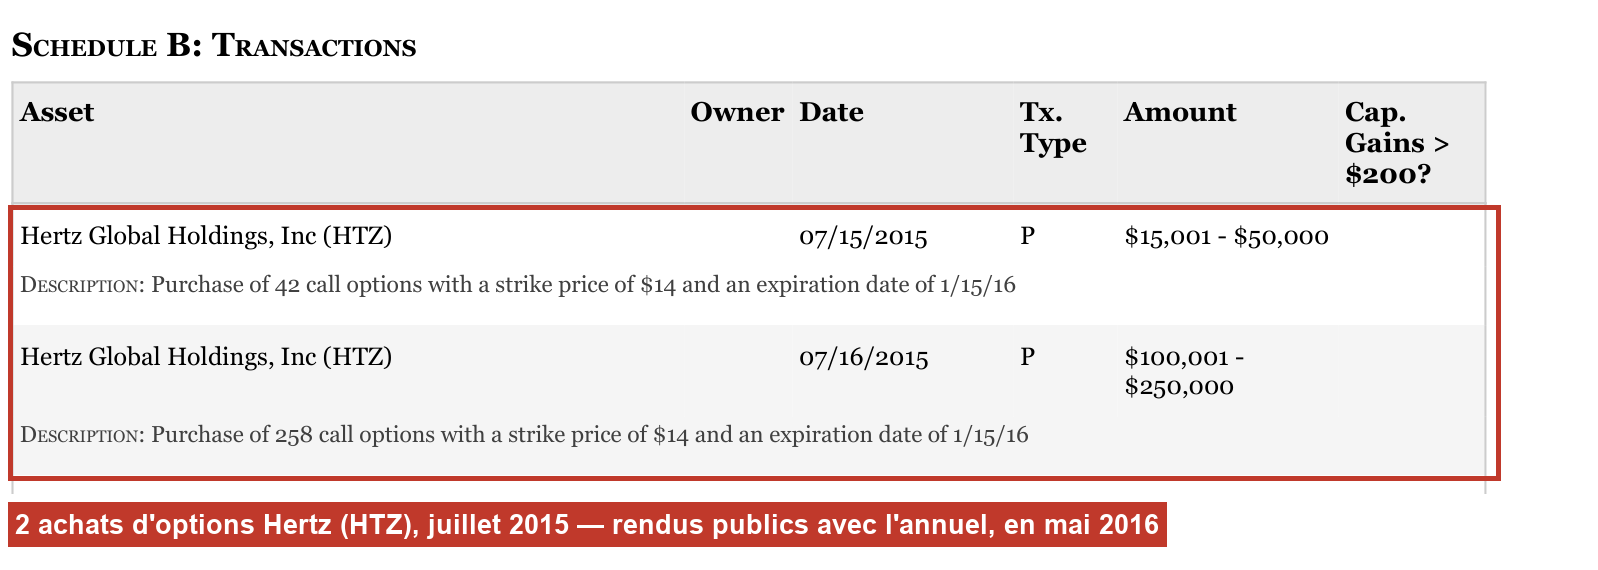
\includegraphics[width=0.92\linewidth,height=44mm,keepaspectratio]{slides/fig_pelosi_schedb.png}}\\[0.8mm]
      {\scriptsize\color{black!60} la Schedule B d'un \textbf{annuel} (Pelosi 2015)
       récapitule les trades de l'année --- souvent déjà déclarés en PTR}
    \end{column}
    \begin{column}{0.52\textwidth}
      \centering
      \begin{tikzpicture}[node distance=2.4mm]
        \node[bande=grisC, text width=7.0cm] (a)
          {\textbf{57\,259} lignes brutes hors PTR (doublons compris)};
        \node[bande=helec, text width=7.0cm, below=of a] (b)
          {doublons et échos des PTR retirés → le net jamais vu en PTR :
           surtout des \textbf{ETF/fonds} \emph{(détail : annexe A5)}};
        \node[rectangle, rounded corners=2pt, draw=alertred, fill=alertred, line width=0.8pt,
              align=center, font=\scriptsize, text width=7.0cm, minimum height=0.62cm, below=of b] (c)
          {\color{white}\textbf{173 vraies actions absentes du signal --- toutes pré-2018}};
        \draw[arr] (a) -- (b); \draw[arr] (b) -- (c);
      \end{tikzpicture}\\[2mm]
      \badgel{warnorange!40}{374 j de délai médian (vs 27 j en PTR)}\\[2mm]
      \choixbox{les transactions hors PTR alimentent le \textbf{patrimoine}
       (vérification), jamais le \textbf{signal} --- découvertes $\sim$1 an trop tard :
       cohérent avec l'anti-look-ahead de l'Étape 1.}
    \end{column}
  \end{columns}
\end{frame}

% ── 4.4 · Cohérence : l'équation et les testables (fusion Coh-1+2+3) ──
\begin{frame}{Cohérence : le test comptable --- patrimoine d'entrée + nos transactions $\overset{?}{=}$ patrimoine de sortie}
  \badgel{okgreen!30}{Question 2 · Cohérence}\hfill{\scriptsize\color{black!55} Chambre uniquement ($\sim$90\,\% du corpus)}\\[1mm]
  \centering
  {\footnotesize \textbf{photo} = le patrimoine déclaré (Schedule A, aux entrées/sorties) ·
   \textbf{flux} = nos transactions --- l'équation ne se teste que si l'on a
   \textbf{les deux photos} :}\\[3mm]
  \resizebox{0.97\textwidth}{!}{%
  \begin{tikzpicture}[node distance=7mm]
    \node[step=grisC, text width=3.1cm, minimum height=1.4cm, font=\footnotesize] (a)
      {\textbf{\large 900}\\{\scriptsize membres passés par la Chambre 2014--2026}};
    \node[step=dataC, text width=3.1cm, minimum height=1.4cm, font=\footnotesize, right=of a] (b)
      {\textbf{\large 149}\\{\scriptsize entrés PUIS sortis\\(cycle complet)}};
    \node[step=helec, text width=3.1cm, minimum height=1.4cm, font=\footnotesize, right=of b] (c)
      {\textbf{\large 106}\\{\scriptsize les DEUX photos réellement déposées}};
    \node[step=okgreen, text width=3.1cm, minimum height=1.4cm, font=\footnotesize, right=of c] (d)
      {\textbf{\large 56}\\{\scriptsize actions cotées des deux côtés → \textbf{testables}}};
    \draw[arr] (a) -- (b); \draw[arr] (b) -- (c); \draw[arr] (c) -- (d);
  \end{tikzpicture}}\\[3mm]
  {\footnotesize la loi elle-même limite l'échantillon : \textbf{439} étaient déjà en
   poste en 2014 (pas de photo d'entrée), \textbf{437} sont encore en poste (pas de
   photo de sortie) ; la moitié des 106 ne détient \textbf{aucune action cotée}}
\end{frame}

% ── 4.5 · Cohérence : le résultat (Coh-4 allégée) ──
\begin{frame}{Cohérence : 87,8\,\% des positions de sortie expliquées --- 3,3\,\% inexpliquées}
  \badgel{okgreen!30}{Question 2 · Cohérence}\hfill{\scriptsize\color{black!55} Chambre uniquement}\\[0.3mm]
  \begin{columns}[c]
    \begin{column}{0.44\textwidth}\centering
      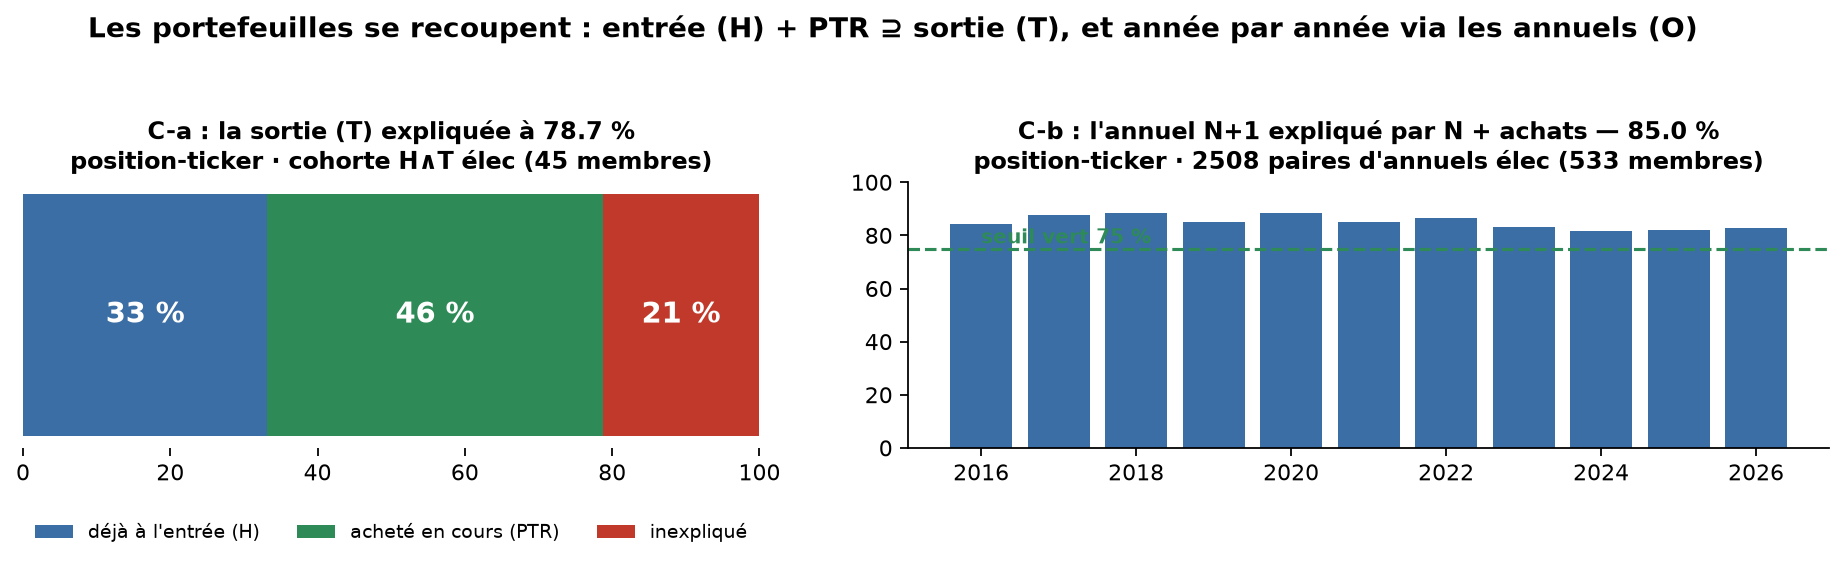
\includegraphics[width=\linewidth,height=0.42\textheight,keepaspectratio]{slides/fig_v1_coherence.png}\\[0.5mm]
      {\scriptsize\color{black!60} premier passage : entrée + achats PTR expliquent
       \textbf{78,7\,\%} des \textbf{1\,371} positions de sortie → \textbf{292}
       inexpliquées}
    \end{column}
    \begin{column}{0.54\textwidth}
      \centering
      \begin{tikzpicture}[node distance=2mm]
        \node[bande=grisC, text width=6.6cm] (a) {\textbf{292 positions inexpliquées} (21,3\,\%) --- instruites \textbf{une par une} :};
        \node[bande=helec, text width=6.6cm, below=of a] (b)
          {\textbf{−125 déclarées AILLEURS} (annuels, sorties, PTR papier)\\
           {\tiny le taux monte : 78,7 → \textbf{87,8\,\%}}};
        \node[bande=dataC, text width=6.6cm, below=of b] (c)
          {\textbf{−122 structurelles} (comptes gérés, petites lignes, ETF exemptés)};
        \node[rectangle, rounded corners=2pt, draw=alertred, fill=alertred, line width=0.8pt,
              align=center, font=\scriptsize, text width=6.6cm, minimum height=0.62cm, below=of c] (d)
          {\color{white}\textbf{45 vraiment inexpliquées = 3,3\,\%} (14 membres)};
        \draw[arr] (a) -- (b); \draw[arr] (b) -- (c); \draw[arr] (c) -- (d);
      \end{tikzpicture}\\[0.6mm]
      \choixbox{chaque position inexpliquée est \textbf{classée par preuve documentaire}
       (table nominative conservée), pas éliminée statistiquement.}\\[0.6mm]
      {\scriptsize\color{black!55} −125 = 74 annuels + 49 sorties + 2 PTR papier ·
       −122 = 59 gérés + 32 $\leq$ 15\,k\$ + 30 ETF + 1 renommage}
    \end{column}
  \end{columns}
\end{frame}

% ── 4.6 · Reconstruire ≠ vérifier (Coh-6 conservée) ──
\begin{frame}{Reconstruire n'est pas vérifier : 9 portefeuilles reconstruits sur 10 restent sans preuve}
  \badgel{okgreen!30}{Question 2 · Cohérence}\hfill{\scriptsize\color{black!55} Chambre uniquement}\\[1mm]
  \centering
  {\footnotesize chacun des \textbf{900} membres reçoit \textbf{un seul statut} --- du
   moins au plus exigeant :}\\[1mm]
  \begin{tikzpicture}[node distance=2mm]
    \node[rectangle, rounded corners=2pt, draw=grisC, fill=grisC!10, line width=0.8pt,
          text width=12.4cm, align=left, font=\scriptsize, inner sep=4.5pt] (r1)
      {\makebox[0.85cm][r]{\normalsize\textbf{20}}\;\; \textbf{hors d'atteinte} --- rien d'exploitable
       (patrimoine 100\,\% non coté, blind trust)};
    \node[rectangle, rounded corners=2pt, draw=dataC, fill=dataC!10, line width=0.8pt,
          text width=12.4cm, align=left, font=\scriptsize, inner sep=4.5pt, below=of r1] (r2)
      {\makebox[0.85cm][r]{\normalsize\textbf{715}}\;\; \textbf{reconstructible partiel} --- au moins
       une photo \textbf{ou} des transactions → des \textbf{morceaux datés}};
    \node[rectangle, rounded corners=2pt, draw=helec, fill=helec!10, line width=0.8pt,
          text width=12.4cm, align=left, font=\scriptsize, inner sep=4.5pt, below=of r2] (r3)
      {\makebox[0.85cm][r]{\normalsize\textbf{109}}\;\; \textbf{reconstructible complet} --- série
       datée de bout en bout\ldots{} mais pas de photo de \textbf{sortie} : \textbf{non testable}};
    \node[rectangle, rounded corners=2pt, draw=okgreen, fill=okgreen, line width=0.8pt,
          text width=12.4cm, align=left, font=\scriptsize, inner sep=4.5pt, below=of r3] (r4)
      {\color{white}\makebox[0.85cm][r]{\normalsize\textbf{56}}\;\; \textbf{vérifiable strict} ---
       les \textbf{deux} photos + actions cotées → l'équation \textbf{réellement testée}
       (le 87,8\,\%)};
  \end{tikzpicture}\\[1.5mm]
  {\scriptsize\color{black!60} 20 + 715 + 109 + 56 = \textbf{900} --- une partition, rien ne se recouvre}\\[1.5mm]
  \choixbox{on affiche le \textbf{périmètre réel du test} (56 membres) plutôt que de
   laisser croire à une vérification universelle --- $\sim$9 reconstruits sur 10 restent
   \textbf{sans preuve}.}
\end{frame}

% ── 4.7 · Corroboration Quiver (fusion S24+S25) ──
\begin{frame}{Corroboration : nous retrouvons $>$\,92\,\% de la base du tiers --- et nous sommes son sur-ensemble}
  \badgel{dataC!30}{Question 3 · Corroboration}\hfill
  {\scriptsize\color{black!60} Quiver = fournisseur commercial, vérité-terrain externe}\\[1mm]
  \begin{columns}[c]
    \begin{column}{0.46\textwidth}\centering
      \begin{tikzpicture}
        \begin{scope}[fill opacity=0.5]
          \fill[helec!35] (0,0) circle (1.42);
          \fill[dataC!35] (1.97,0) circle (1.42);
        \end{scope}
        \draw[helec, line width=1.1pt] (0,0) circle (1.42);
        \draw[dataC, line width=1.1pt] (1.97,0) circle (1.42);
        \node[font=\footnotesize\bfseries, text=helec] at (-0.9,1.62) {NOUS (169\,000)};
        \node[font=\footnotesize\bfseries, text=dataC] at (2.9,1.62) {QUIVER};
        \node[align=center, font=\scriptsize, text width=1.5cm] at (-0.75,0)
          {\textbf{nous seuls}\\{\color{helec}\textbf{$\approx$\,26\,500}}\\{\tiny (sur-ensemble)}};
        \node[align=center, font=\scriptsize, text width=1.3cm] at (0.985,0)
          {\textbf{retrouvés}\\\textbf{93,5\,\%} Ch.\\\textbf{92,1\,\%} Sén.};
        \node[align=center, font=\scriptsize, text width=1.5cm] at (2.72,0)
          {\textbf{Quiver seul}\\\textbf{38} → {\color{alertred}\textbf{27+11}}\\{\tiny vrais trous documentés}};
      \end{tikzpicture}\\[1mm]
      {\scriptsize\color{black!60} au niveau (élu, ticker, sens) : \textbf{93,5\,\% /
       92,1\,\%} des combinaisons \emph{de Quiver} sont retrouvées \emph{chez nous}}
    \end{column}
    \begin{column}{0.52\textwidth}\footnotesize
      \textbf{trois crans de strictesse} --- on serre la vis :\\[1mm]
      {\scriptsize
      \badge{helec}{1 · exister} même élu, même titre, même sens\\[0.8mm]
      \badge{helec}{2 · dater} même date ($\leq$10 j) --- appariés un à un\\[0.8mm]
      \badge{helec}{3 · concorder} sens \textbf{96,8\,\%} · montant \textbf{94,2\,\%} (Chambre)}\\[2.5mm]
      \choixbox{Quiver est une \textbf{vérité-terrain jamais réinjectée} : il
       \textbf{mesure} la table, ne la remplit jamais --- et en cas de désaccord de
       date, \textbf{le PDF officiel arbitre toujours} (annexe A6).}
    \end{column}
  \end{columns}
\end{frame}

% ── 4.8 · Les autres preuves + le principe (S26 resserrée) ── (ferme l'étape)
\begin{frame}{Cinq preuves de plus, un principe : rien n'est réinjecté}
  \badgel{dataC!30}{Question 3 · Corroboration}\\[1mm]
  \centering
  \begin{minipage}[t]{0.32\textwidth}
    \carte{helec}{Univers officiel}{index du \emph{House Clerk} re-traversé :
      \textbf{100\,\%} des \textbf{8\,252 PTR} traités --- parsés, lus par OCR, ou
      écartés par règle écrite}
  \end{minipage}\hfill
  \begin{minipage}[t]{0.32\textwidth}
    \carte{okgreen}{Collectes indépendantes}{deux projets tiers ayant collecté les
      mêmes sources : \textbf{100\,\%} et \textbf{99,5\,\%} de leurs lignes retrouvées
      chez nous (+ un agrégateur tiers en triangulation)}
  \end{minipage}\hfill
  \begin{minipage}[t]{0.32\textwidth}
    \carte{alertred}{Re-run reproductible}{\textbf{368} signatures de fichiers figées :
      chaque nouvelle exécution doit reproduire les tables livrées \textbf{à l'octet
      près} --- aucune régression silencieuse}
  \end{minipage}\\[4mm]
  \colorbox{black!6}{\parbox{0.84\textwidth}{\footnotesize\centering\vspace{0.8mm}
    \textbf{le principe} --- aucune source externe n'est \textbf{réinjectée} dans les
    tables : elles ne servent qu'à \textbf{mesurer} ce qu'on a\vspace{0.8mm}}}\\[3mm]
  \repband{rien raté (173 actions résiduelles côté patrimoine · 27 + 11 vrais trous face
   au tiers) · cohérent dedans (87,8\,\% des positions expliquées) · sur-ensemble dehors
   ($>$\,92\,\% de la base du tiers retrouvée).}
\end{frame}

\section{Étape 5 · Le livrable}
% ── intercalaire Étape 5 ──
\begin{frame}[plain]
  \centering
  \vspace{14mm}
  {\Large\bfseries\color{black!80} Étape 5 --- Le livrable}\\[8mm]
  \begin{tikzpicture}[scale=1.0, every node/.style={transform shape}]
\node[rectangle, rounded corners=2.5pt, draw=okgreen, fill=okgreen!10, line width=0.8pt, text width=2.35cm, minimum height=1.05cm, align=center, font=\scriptsize] (b1) at (1.325,0) {\color{okgreen}\checkmark~\textbf{1 · \mbox{Donnée brute}}};
\draw[arr] (2.65,0) -- (3.07,0);
\node[rectangle, rounded corners=2.5pt, draw=okgreen, fill=okgreen!10, line width=0.8pt, text width=2.35cm, minimum height=1.05cm, align=center, font=\scriptsize] (b2) at (4.395,0) {\color{okgreen}\checkmark~\textbf{2 · Pipeline}};
\draw[arr] (5.72,0) -- (6.14,0);
\node[rectangle, rounded corners=2.5pt, draw=okgreen, fill=okgreen!10, line width=0.8pt, text width=2.35cm, minimum height=1.05cm, align=center, font=\scriptsize] (b3) at (7.465,0) {\color{okgreen}\checkmark~\textbf{3 · Enrichir}};
\draw[arr] (8.79,0) -- (9.209999999999999,0);
\node[rectangle, rounded corners=2.5pt, draw=okgreen, fill=okgreen!10, line width=1.3pt, text width=2.75cm, minimum height=1.05cm, align=center, font=\scriptsize] (b4) at (10.735,0) {\color{okgreen}\checkmark~\textbf{4 · \mbox{VÉRIFICATION}}};
\draw[arr] (12.259999999999998,0) -- (12.679999999999998,0);
\node[rectangle, rounded corners=2.5pt, draw=okgreen, fill=okgreen, line width=0.8pt, text width=2.35cm, minimum height=1.05cm, align=center, font=\scriptsize] (b5) at (14.004999999999999,0) {\color{white}\textbf{5 · Livrable}};
\end{tikzpicture}\\[9mm]
  {\normalsize\itshape\color{black!55} Qu'est-ce qu'on livre, et avec quelles limites ?}
\end{frame}

% ── 5.1 · L'entonnoir (S27 re-titrée) ──
\begin{frame}{De 169\,000 à 134\,464 : on ne retire que l'avéré inutilisable}
  \begin{columns}[T]
    \begin{column}{0.58\textwidth}
      \centering
      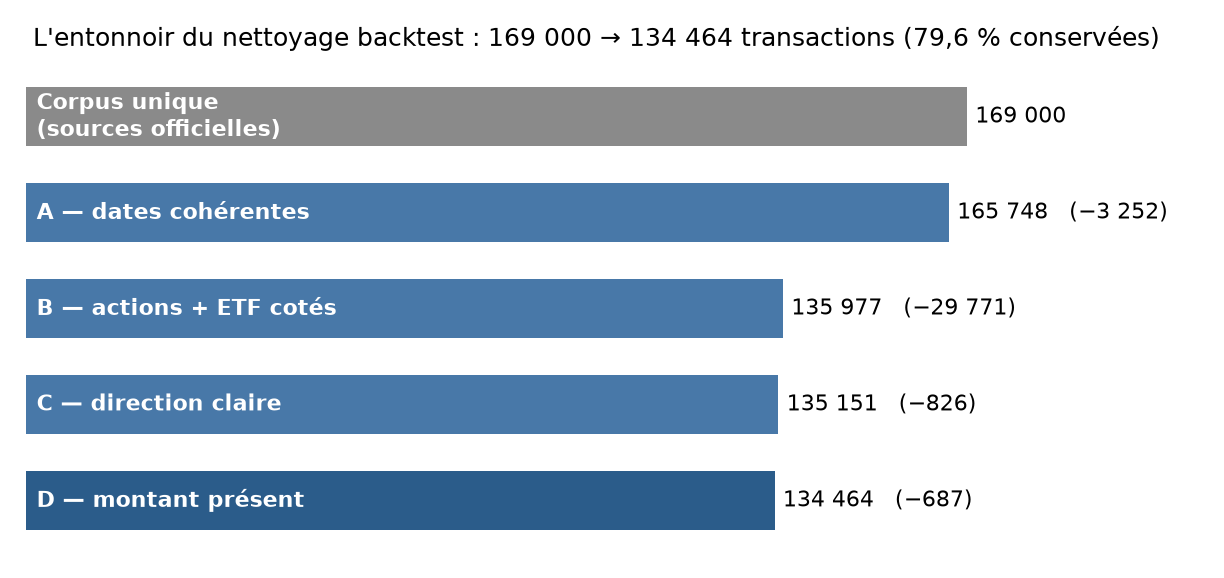
\includegraphics[width=\linewidth]{quality/entonnoir_backtest.png}
    \end{column}
    \begin{column}{0.40\textwidth}
      {\footnotesize quatre portes objectives --- \textbf{169\,000 → 134\,464}
       (79,6\,\% conservées) :}\\[1.5mm]
      {\scriptsize
      \textbf{A --- dates cohérentes} : \textbf{−3\,252}\\[0.8mm]
      \textbf{B --- actions + ETF cotés} (un backtest exige un prix de marché) :
        \textbf{−29\,771}\\[0.8mm]
      \textbf{C --- direction claire} (achat ou vente) : \textbf{−826}\\[0.8mm]
      \textbf{D --- montant présent} : \textbf{−687}}\\[2mm]
      \colorbox{okgreen!10}{\parbox{0.96\linewidth}{\scriptsize
        \textbf{\textcolor{okgreen}{sauvetage « ticker-first »}} --- \textbf{21\,878}
        lignes à case « type d'actif » vide \textbf{gardées} : le \textbf{ticker coté}
        fait foi, pas la case déclarée}}
    \end{column}
  \end{columns}
  \vspace{1.5mm}
  \centering
  \choixbox{on ne retire que l'\textbf{avéré inutilisable} ; le doute est
   \textbf{flagué, jamais retiré} (late filing 12,2\,\%, délistés, lots multi-comptes)
   --- la recherche décide.}
\end{frame}

% ── 5.2 · Du symbole au prix (S27b allégée + réconciliation) ──
\begin{frame}{Du symbole au prix : 118\,029 trades valorisables --- et un biais de survie assumé}
  \begin{columns}[c]
    \begin{column}{0.52\textwidth}\centering
      \begin{tikzpicture}[node distance=3.2mm]
        \node[bande=grisC, text width=6.4cm, minimum height=1.0cm] (a)
          {\textbf{4\,618} symboles distincts dans la table};
        \node[bande=helec, text width=6.4cm, minimum height=1.0cm, below=of a] (b)
          {\textbf{3\,350} servis par Yahoo\\{\scriptsize −1\,268 \textbf{délistés sans successeur coté}}};
        \node[bande=okgreen, text width=6.4cm, minimum height=1.0cm, below=of b] (c)
          {\textbf{3\,289} exploitables\\{\scriptsize −61 séries corrompues (garde-fous)}};
        \draw[arr] (a) -- (b); \draw[arr] (b) -- (c);
      \end{tikzpicture}
    \end{column}
    \begin{column}{0.46\textwidth}
      \badge{okgreen}{118\,029 trades avec un prix fiable ($\approx$ 88 \%)}\\[1.5mm]
      {\scriptsize\color{black!60} même valeur numérique que le taux de cohérence de
       l'Étape 4 : \textbf{pure coïncidence}, aucun lien}\\[2.5mm]
      \colorbox{warnorange!12}{\parbox{0.96\linewidth}{\footnotesize\vspace{0.5mm}
        \textbf{\textcolor{warnorange}{biais de survie assumé}} --- un titre mort depuis
        (faillite, rachat sans successeur) ne peut plus être valorisé :
        couverture \textbf{74\,\%} en 2014 → \textbf{99\,\%} en 2026\vspace{0.5mm}}}\\[2mm]
      \choixbox{la limite est \textbf{écrite}, pas cachée --- les lignes non couvertes
       \textbf{restent} dans la table, flaguées.}
    \end{column}
  \end{columns}
  \vspace{1.5mm}
  \centering
  {\scriptsize\color{black!55} note : le moteur d'analyse aval filtre l'année du trade
   à 2013--2026 → il travaille sur \textbf{134\,429} lignes (134\,464 − 35 trades à
   année aberrante, coquilles fidèlement transcrites)}
\end{frame}

% ── 5.3 · La table livrée (S28 allégée) ──
\begin{frame}{La table livrée : 134\,464 lignes × 36 colonnes, traçables au document près}
  \centering
  \colorbox{helec}{\parbox{0.9\textwidth}{\scriptsize\color{white}\centering\vspace{0.6mm}
    la table de recherche --- \textbf{134\,464 lignes × 36 colonnes} ·
    372 élus · chaque ligne traçable à son document source\vspace{0.6mm}}}\\[1.2mm]
  {\footnotesize
  \begin{tabular}{@{}llllrl@{}}
    \toprule
    \textbf{membre} & \textbf{ticker} & \textbf{sens} & \textbf{transaction} & \textbf{montant \$} & \textbf{secteur} \\
    \midrule
    Bob Gibbs & INTC & buy & 2014-12-30 & 8\,000,5 & Info.\ Tech. \\
    Greg Gianforte & BBAVY & sell & 2018-12-12 & 32\,500,5 & Cons.\ Staples \\
    Kim Schrier & AAPL & buy & 2021-11-15 & 375\,000,5 & Info.\ Tech. \\
    Tim Moore & HOG & buy & 2025-12-09 & 32\,500,5 & Cons.\ Discr. \\
    \bottomrule
  \end{tabular}}\\[0.6mm]
  {\scriptsize\color{black!60} 4 lignes réelles --- le montant est le \textbf{milieu
   exact de la fourchette} (d'où les « ,5 »)}\\[1.5mm]
  \begin{columns}[T]
    \begin{column}{0.52\textwidth}
      {\footnotesize\textbf{les 36 colonnes, en 3 familles}}\\[0.3mm]
      {\scriptsize · \textbf{qui \& quand} --- élu, parti \& commissions à la date du
        trade, 2 dates\\[0.3mm]
       · \textbf{quoi \& combien} --- ticker, secteur, ETF, montant (99,4\,\%)\\[0.3mm]
       · \textbf{flags \& traçabilité} --- document source par ligne}
    \end{column}
    \begin{column}{0.44\textwidth}
      {\footnotesize\textbf{limites écrites, dans le livrable}}\\[0.3mm]
      {\scriptsize · \textbf{582 PTR manuscrits} écartés (7,1\,\% de l'index)\\
       · \textbf{biais de survie} prix (slide précédente)\\
       · composition : Chambre \textbf{91,3\,\%} · achats \textbf{50,8\,\%}}
    \end{column}
  \end{columns}
\end{frame}

% ── FIN · La couche données en 4 chiffres (S29, légendes suffixées) ──
\begin{frame}{La couche données, en quatre chiffres}
  \centering
  \vspace{2mm}
  \begin{tikzpicture}[scale=1.0, every node/.style={transform shape}]
\node[rectangle, rounded corners=2.5pt, draw=okgreen, fill=okgreen!10, line width=0.8pt, text width=2.35cm, minimum height=1.05cm, align=center, font=\scriptsize] (b1) at (1.325,0) {\color{okgreen}\checkmark~\textbf{1 · \mbox{Donnée brute}}};
\draw[arr] (2.65,0) -- (3.07,0);
\node[rectangle, rounded corners=2.5pt, draw=okgreen, fill=okgreen!10, line width=0.8pt, text width=2.35cm, minimum height=1.05cm, align=center, font=\scriptsize] (b2) at (4.395,0) {\color{okgreen}\checkmark~\textbf{2 · Pipeline}};
\draw[arr] (5.72,0) -- (6.14,0);
\node[rectangle, rounded corners=2.5pt, draw=okgreen, fill=okgreen!10, line width=0.8pt, text width=2.35cm, minimum height=1.05cm, align=center, font=\scriptsize] (b3) at (7.465,0) {\color{okgreen}\checkmark~\textbf{3 · Enrichir}};
\draw[arr] (8.79,0) -- (9.209999999999999,0);
\node[rectangle, rounded corners=2.5pt, draw=okgreen, fill=okgreen!10, line width=1.3pt, text width=2.75cm, minimum height=1.05cm, align=center, font=\scriptsize] (b4) at (10.735,0) {\color{okgreen}\checkmark~\textbf{4 · \mbox{VÉRIFICATION}}};
\draw[arr] (12.259999999999998,0) -- (12.679999999999998,0);
\node[rectangle, rounded corners=2.5pt, draw=okgreen, fill=okgreen!10, line width=0.8pt, text width=2.35cm, minimum height=1.05cm, align=center, font=\scriptsize] (b5) at (14.004999999999999,0) {\color{okgreen}\checkmark~\textbf{5 · Livrable}};
\end{tikzpicture}\\[6mm]
  \tuile{helec}{100\,\%}{de l'univers officiel\\(8\,252 PTR) traité}\hfill
  \tuile{grisC}{169\,000}{transactions uniques,\\identifiées à 100\,\%}\hfill
  \tuile{alertred}{$>$\,92\,\%}{base du tiers retrouvée · 87,8\,\%\\des positions expliquées}\hfill
  \tuile{okgreen}{134\,464 $\times$ 36}{lignes × colonnes,\\limites écrites}\\[4mm]
  {\footnotesize une couche données \textbf{vérifiée de l'intérieur et de l'extérieur} ---
   sur laquelle bâtir en connaissant ses limites}\\[2mm]
  \repband{une table 134\,464 × 36 · 79,6\,\% du corpus · limites écrites.}
\end{frame}

% ══════════════════ ANNEXES ══════════════════
\appendix
\section{Annexes}

\begin{frame}[plain]
  \centering\vfill
  {\color{helec!85}\large\textbf{Annexes}}\\[3.5mm]
  {\color{black!88}\fontsize{29}{33}\selectfont\textbf{La réserve pour questions}}\\[4mm]
  {\color{helec!45}\rule{0.30\textwidth}{1.2pt}}\\[4mm]
  {\color{black!55}\large A1--A7 : documents exemples · détails des cascades · cas particuliers}
  \vfill
\end{frame}

% ── A1 · Le PTR lisible en grand (ex-S5a) ──
\begin{frame}{A1 --- Le document lisible : un PTR électronique}
  \begin{columns}[T]
    \begin{column}{0.55\textwidth}\centering
      \fcolorbox{helec}{white}{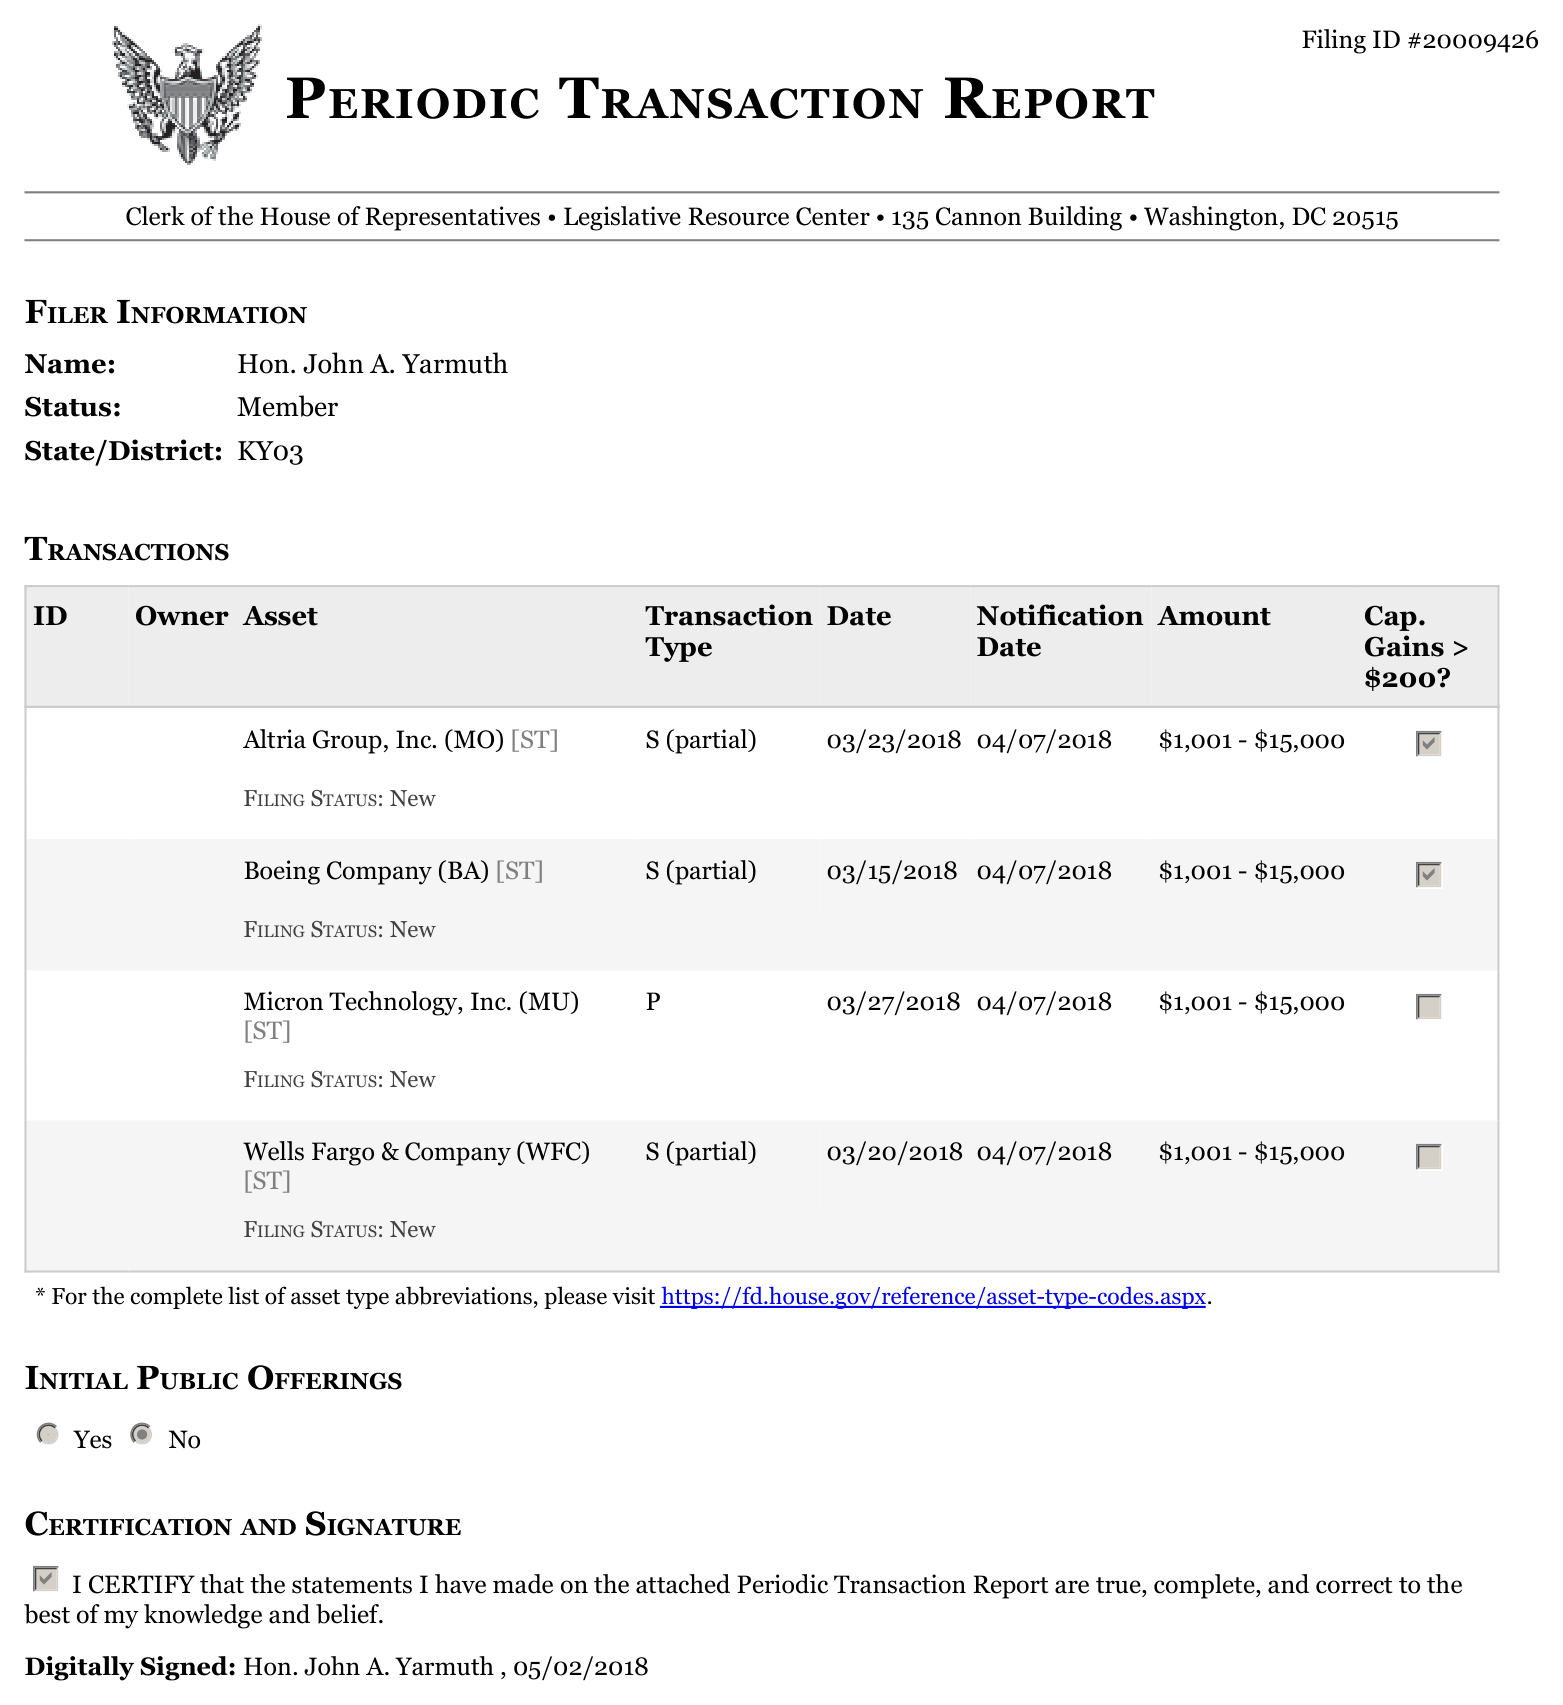
\includegraphics[width=0.92\linewidth,height=64mm,keepaspectratio]{slides/fig_ptr_digital.png}}\\[0.5mm]
      {\scriptsize\color{black!60} PTR électronique complet (Hon.\ John A.\ Yarmuth, KY03)}
    \end{column}
    \begin{column}{0.43\textwidth}
      {\footnotesize
      · un PDF \textbf{lisible par machine} (couche texte)\\[1.5mm]
      · le ticker est imprimé \textbf{entre parenthèses} : \co{(BA)},
        le type d'actif entre crochets : \co{[ST]}\\[1.5mm]
      · deux dates par ligne (trade / notification --- cette dernière est jetée)
        + fourchette de montant\\[1.5mm]
      · \textbf{7\,996} lignes au montant coupé en deux, recollées avant lecture}
    \end{column}
  \end{columns}
\end{frame}

% ── A2 · Captures détaillées (ex-S2b + S7b) ──
\begin{frame}{A2 --- L'index annuel de la Chambre, la recherche eFD du Sénat}
  \begin{columns}[T]
    \begin{column}{0.40\textwidth}\centering
      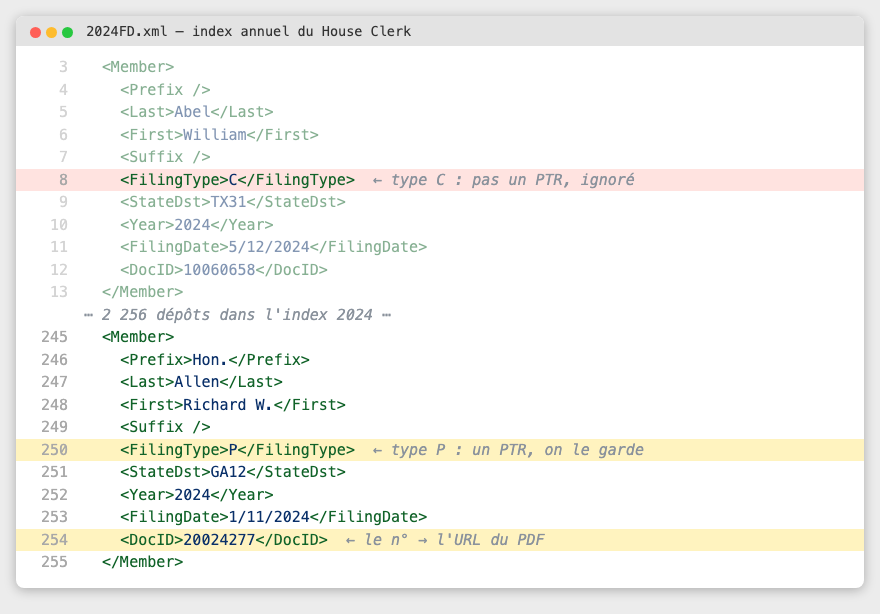
\includegraphics[width=\linewidth]{slides/fichier_index_xml.png}\\[0.5mm]
      {\scriptsize\color{black!60} l'index annuel : un bloc par dépôt
       (archive \co{2024FD.zip} → \co{2024FD.xml})}
    \end{column}
    \begin{column}{0.29\textwidth}\centering
      \fcolorbox{black!25}{white}{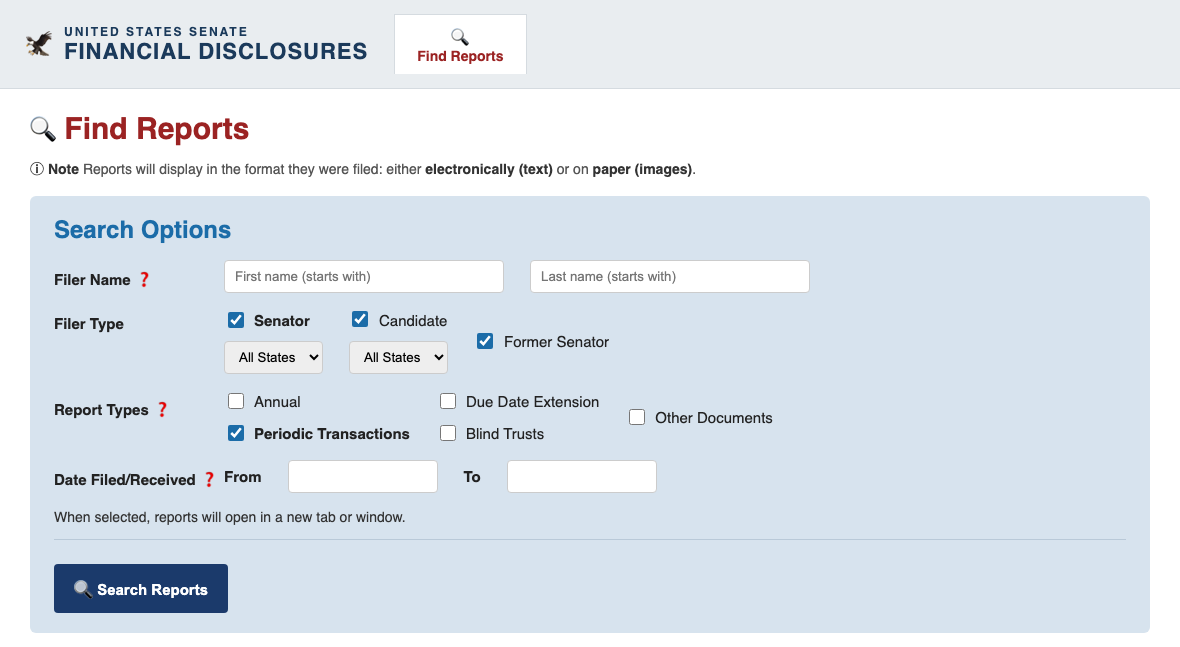
\includegraphics[width=0.89\linewidth]{slides/site_senate_form.png}}\\[0.5mm]
      {\scriptsize\color{black!60} eFD : on coche \textbf{Senator} × \textbf{PTR}}
    \end{column}
    \begin{column}{0.29\textwidth}\centering
      \fcolorbox{black!25}{white}{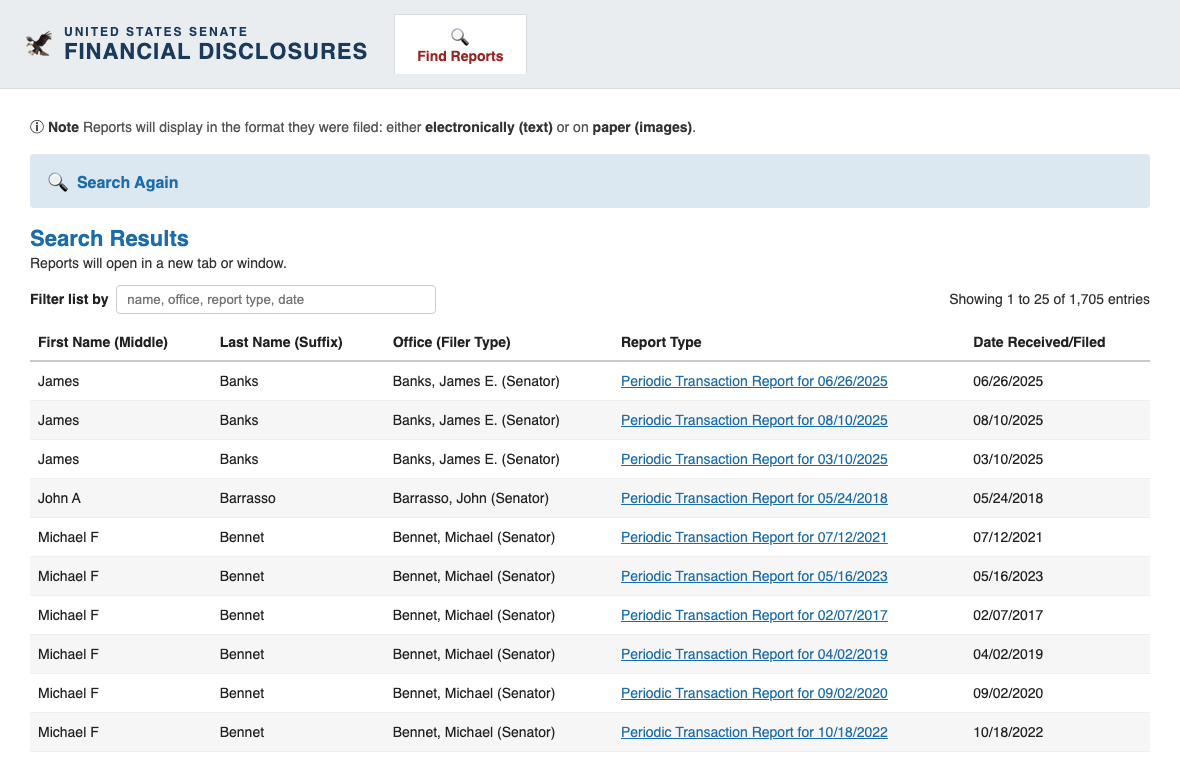
\includegraphics[width=0.89\linewidth]{slides/site_senate_results.png}}\\[0.5mm]
      {\scriptsize\color{black!60} la liste de dépôts, un lien chacun ---
       chaque dépôt s'ouvre en HTML ou en scan}
    \end{column}
  \end{columns}
  \vspace{2mm}
  \centering
  {\scriptsize\color{black!60} zéro échec silencieux : 102 dépôts sans transaction
   retenue, tous consignés (vides réels, amendements sans ligne, échecs tracés)}
\end{frame}

% ── A3 · La matrice des sections (ex-Compl 2/5) ──
\begin{frame}{A3 --- Le même formulaire, des sections en commun}
  \centering
  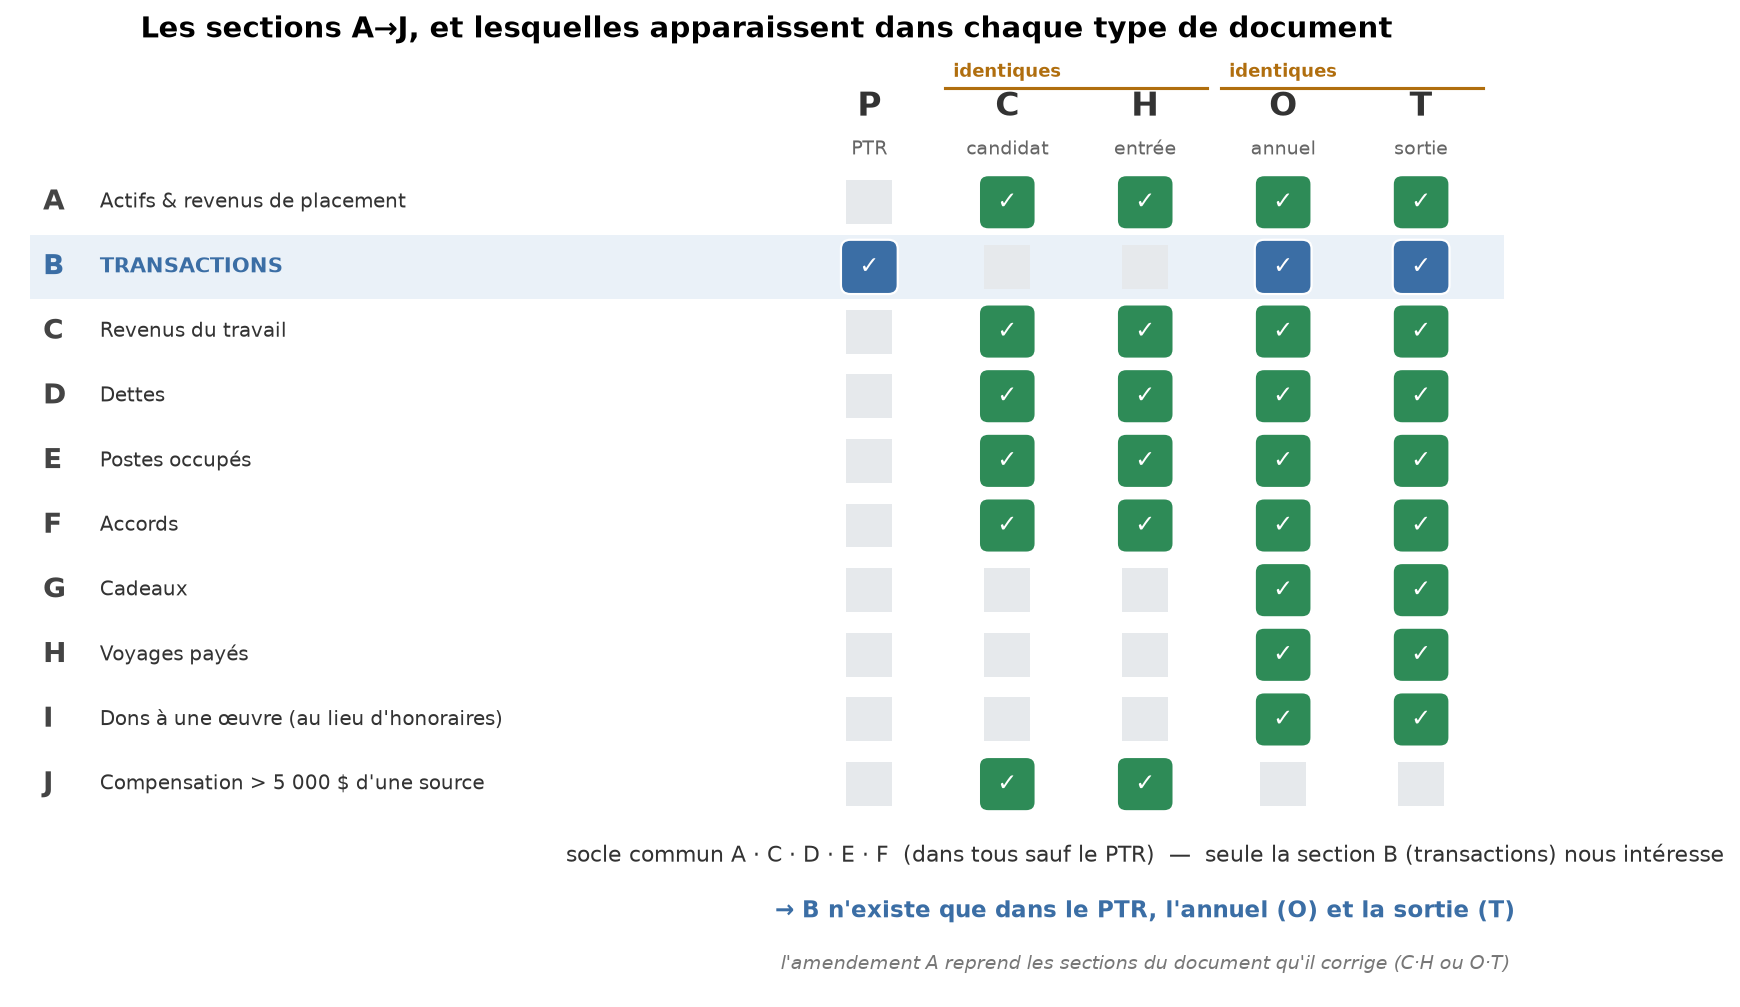
\includegraphics[height=0.61\textheight]{slides/fig_sections_matrix.png}\\[0.5mm]
  {\footnotesize la \textbf{section B} = les transactions ; le reste est un socle
   commun, la \textbf{A} (patrimoine) sert à \emph{vérifier}}
\end{frame}

% ── A4 · Les administratifs + le blind trust (ex-Compl 5/5) ──
\begin{frame}{A4 --- Les types administratifs, et le cas à part}
  \centering
  {\footnotesize cinq types \textbf{sans aucune transaction} :}\\[1.5mm]
  \begin{columns}[T]
    \begin{column}{0.19\textwidth}\centering
      \fcolorbox{black!30}{white}{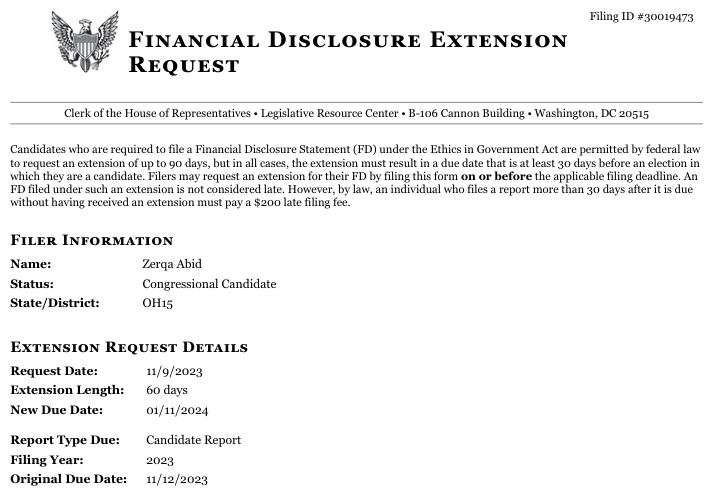
\includegraphics[width=0.88\linewidth,height=20mm,keepaspectratio]{slides/ftype_x.png}}\\[0.6mm]
      {\scriptsize\textbf{X --- Extension}\\demande de délai}
    \end{column}
    \begin{column}{0.19\textwidth}\centering
      \fcolorbox{black!30}{white}{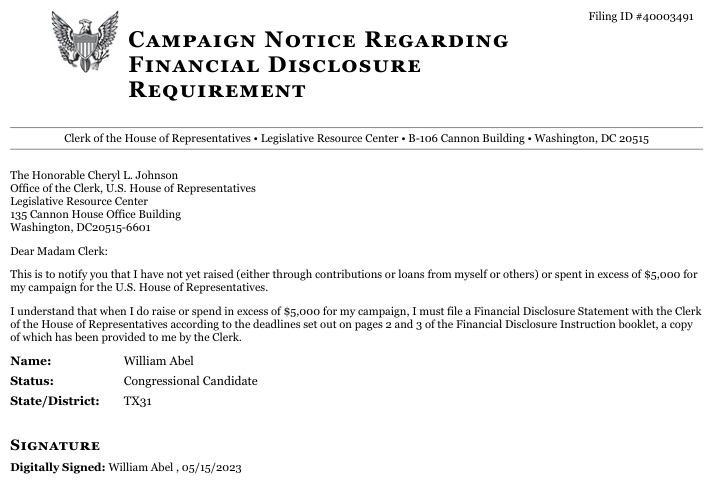
\includegraphics[width=0.88\linewidth,height=20mm,keepaspectratio]{slides/ftype_d.png}}\\[0.6mm]
      {\scriptsize\textbf{D --- Campaign Notice}\\« \textless{} 5\,000 \$ »}
    \end{column}
    \begin{column}{0.19\textwidth}\centering
      \fcolorbox{black!30}{white}{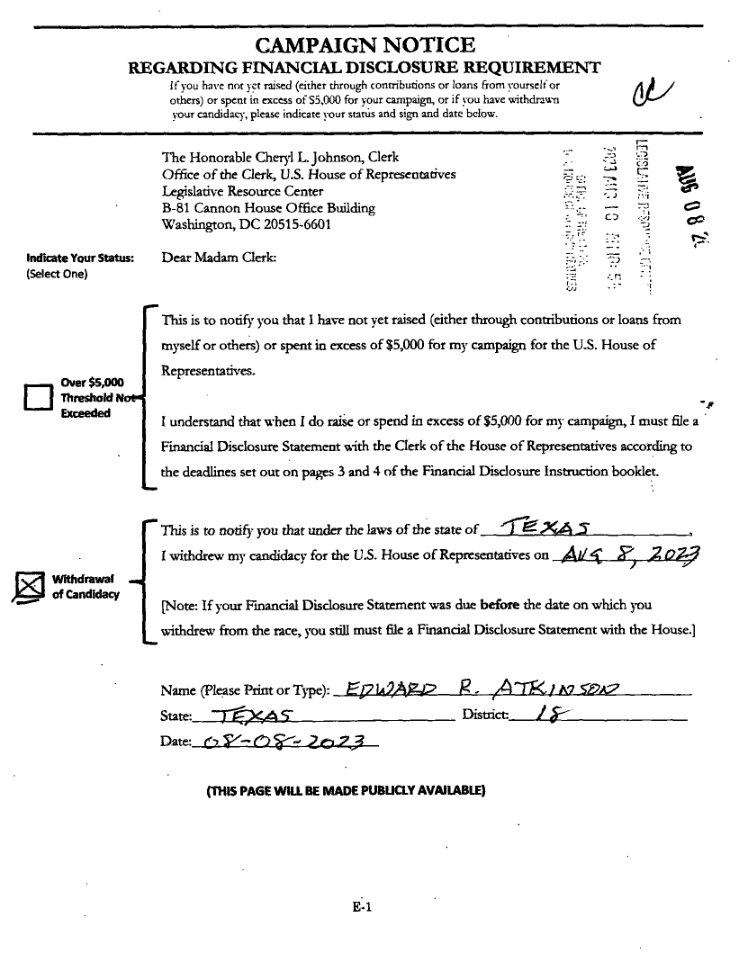
\includegraphics[width=0.88\linewidth,height=20mm,keepaspectratio]{slides/ftype_w.png}}\\[0.6mm]
      {\scriptsize\textbf{W --- idem, papier}\\(ou retrait)}
    \end{column}
    \begin{column}{0.19\textwidth}\centering
      \fcolorbox{black!30}{white}{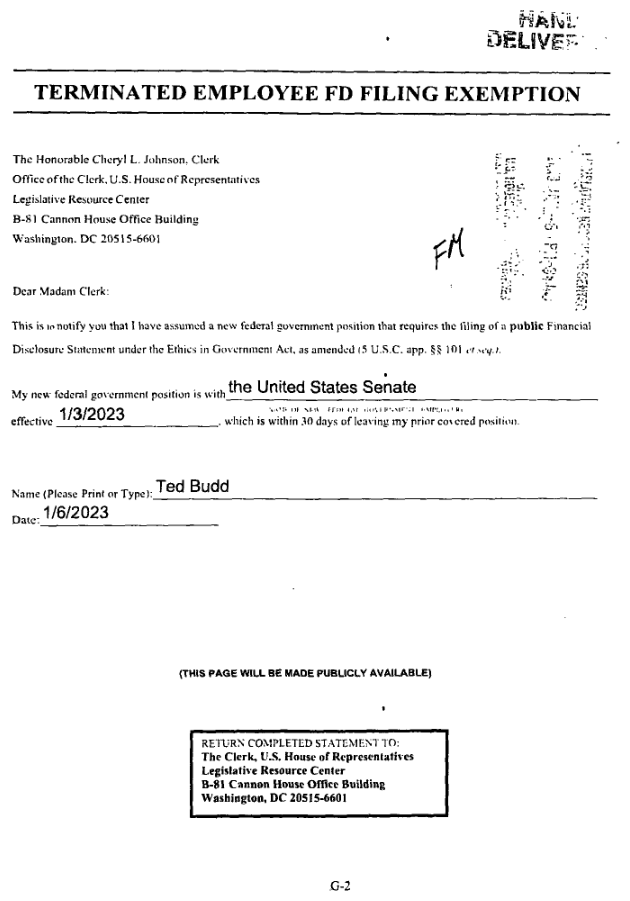
\includegraphics[width=0.88\linewidth,height=20mm,keepaspectratio]{slides/ftype_e.png}}\\[0.6mm]
      {\scriptsize\textbf{E --- Exemption}\\départ, poste fédéral}
    \end{column}
    \begin{column}{0.19\textwidth}\centering
      \fcolorbox{black!30}{white}{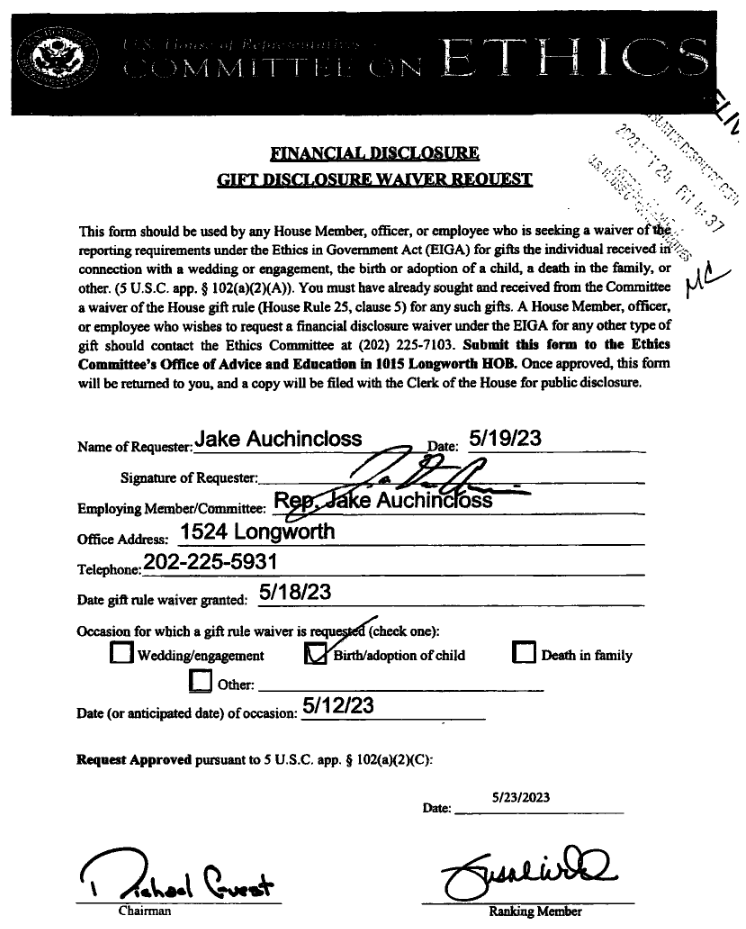
\includegraphics[width=0.88\linewidth,height=20mm,keepaspectratio]{slides/ftype_g.png}}\\[0.6mm]
      {\scriptsize\textbf{G --- Gift Waiver}\\dérogation cadeau}
    \end{column}
  \end{columns}
  \vspace{2.5mm}
  \begin{columns}[c]
    \begin{column}{0.14\textwidth}\centering
      \fcolorbox{alertred}{white}{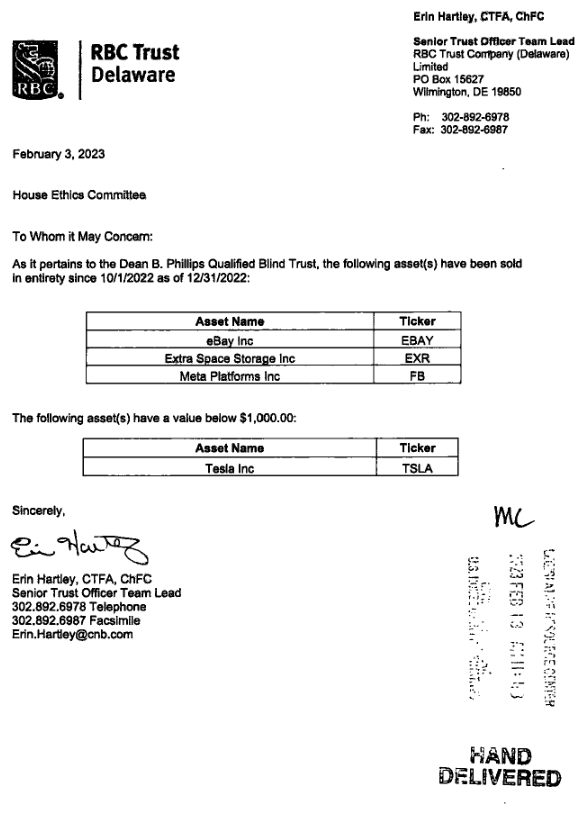
\includegraphics[width=0.86\linewidth,height=19mm,keepaspectratio]{slides/ftype_b.png}}
    \end{column}
    \begin{column}{0.82\textwidth}
      \colorbox{alertred!10}{\parbox{0.97\linewidth}{\footnotesize\raggedright\vspace{0.5mm}
        \textbf{\textcolor{alertred}{B --- Blind Trust}} (23 dépôts) : la banque du
        \emph{trust} liste de vraies ventes, mais \textbf{pas décidées par l'élu} :
        la fiducie aveugle.\vspace{0.5mm}}}
    \end{column}
  \end{columns}
  \vspace{2mm}
  {\scriptsize\color{black!60} et les candidats \textbf{C} : 10\,105 dépôts, 77\,\%
   jamais élus --- une photo de patrimoine qui peut servir de photo d'entrée}
\end{frame}

% ── A5 · Le gain net O/A/T (ex-Coh-5, ré-ancré) ──
\begin{frame}{A5 --- Ce que les O/A/T ajoutent : du patrimoine, pas du signal}
  \centering
  {\footnotesize une fois doublons \textbf{et} échos des PTR retirés, il reste dans les
   annuels (O), sorties (T) et amendements (A) :}\\[3.5mm]
  \tuile{okgreen}{26\,115}{trades jamais vus\\dans un PTR}\hfill
  \tuile{dataC}{22\,216}{via les annuels O}\hfill
  \tuile{dataC}{3\,899}{via sorties T\\+ amendements A}\hfill
  \tuile{grisC}{374 j}{délai médian\\trade → publication}\\[3.5mm]
  \colorbox{alertred}{\parbox{0.92\textwidth}{\footnotesize\color{white}\centering
    ces trades \textbf{comblent des trous du portefeuille} (l'élu oublie son PTR mais
    l'inscrit à l'annuel) --- découverts \textbf{$\sim$1 an trop tard} : ils nourrissent
    le \textbf{patrimoine}, jamais le \textbf{signal}}}\\[2mm]
  {\scriptsize\color{black!55} les 26\,115 sont surtout des \textbf{ETF/fonds cotés} ---
   les vraies \textbf{actions} manquantes au signal = \textbf{173}, toutes pré-2018}\\[1.5mm]
  {\scriptsize\color{black!55} ⚠ ne pas confondre : \textbf{26\,115} (net hors-PTR,
   cohérence interne) $\neq$ \textbf{$\approx$\,26\,500} (combinaisons présentes chez
   nous et absentes chez Quiver, corroboration) --- source : audit patrimoine Chambre,
   table de flux nette (lignée v1-house)}
\end{frame}

% ── A6 · Les dates arbitrées au PDF (ex-S25 détail) ──
\begin{frame}{A6 --- Qui a raison sur les dates ? Le PDF officiel arbitre toujours}
  \centering
  {\footnotesize pour un même (élu, ticker, sens), quand notre date et celle de Quiver
   divergent dans un même dépôt, \textbf{545 candidats} méritent l'œil → on
   \textbf{rouvre le PDF} :}\\[2mm]
  {\footnotesize
  \begin{tabular}{@{}>{\raggedright\arraybackslash}p{0.34\linewidth}>{\raggedright\arraybackslash}p{0.24\linewidth}>{\raggedright\arraybackslash}p{0.30\linewidth}@{}}
    \toprule
    \textbf{le PDF montre…} & \textbf{exemple réel} & \textbf{traitement} \\
    \midrule
    coquille du déposant, prouvable & \ttfamily 3031-04-30 & corrigée → 2021 \\[0.6mm]
    coquille littérale & \ttfamily 01/35/22 & \textcolor{okgreen}{\textbf{transcrite telle quelle}} \\[0.6mm]
    notre OCR s'est trompé & Khanna/COST \ttfamily 09-31 & re-lue au PDF → \ttfamily 08-16 \\[0.6mm]
    désaccord Quiver & McCaul/GOOGL $\Delta$11 j & arbitré au PDF \\
    \bottomrule
  \end{tabular}}\\[2.5mm]
  {\scriptsize\color{black!60} principe : le \textbf{PDF officiel} arbitre toujours ---
   on reste fidèle à la source, même à ses coquilles littérales}
\end{frame}

% ── A7 · Détails : ETF, cascade secteur, couverture entrées/sorties, pièges identité ──
\begin{frame}{A7 --- Détails : les 11 ETF, la couverture des entrées/sorties, les pièges d'identité}
  \begin{columns}[T]
    \begin{column}{0.48\textwidth}\footnotesize
      \textbf{11 secteurs GICS → 11 ETF} \emph{Select Sector SPDR} :\\[1mm]
      {\scriptsize\ttfamily
      Energy→XLE · Materials→XLB · Industrials→XLI · Cons.\ Discr.→XLY ·
      Cons.\ Staples→XLP · Health Care→XLV · Financials→XLF · Info.\ Tech.→XLK ·
      Comm.\ Services→XLC · Utilities→XLU · Real Estate→XLRE}\\[2.5mm]
      \textbf{cascade secteur} : yfinance (factuel) → LLM contraint GICS → overrides
      manuels\\[2.5mm]
      \textbf{pièges d'identité réels, réparés} : l'homonyme Bob Casey
      (\co{C000228} → \co{C001070}) · 42 lignes d'Angie Craig sans identifiant,
      réparées à la lecture
    \end{column}
    \begin{column}{0.48\textwidth}\footnotesize
      \textbf{couverture des entrées/sorties (Chambre)} :\\[1mm]
      {\scriptsize
      \begin{tabular}{@{}p{0.30\linewidth} p{0.60\linewidth}@{}}
        \toprule
        \textbf{470 entrées} depuis 2014 & 82\,\% ont déposé un \textbf{H} (photo
          d'entrée) · 16\,\% un \textbf{C} à la place → \textbf{98\,\% couverts} \\
        \midrule
        \textbf{463 sorties} définitives & 81\,\% ont déposé un \textbf{T} (photo de
          sortie) ; les 86 sans T : partis au Sénat/exécutif (dispensés), décès \\
        \bottomrule
      \end{tabular}}\\[1.5mm]
      {\scriptsize la photo d'entrée : \textbf{252} ancrés par un H · \textbf{32} par
       un C = \textbf{284} portefeuilles d'entrée datés}
    \end{column}
  \end{columns}
\end{frame}

\end{document}
